\documentclass[a4paper,11pt]{article}
% \pdfoutput=1 % if your are submitting a pdflatex (i.e. if you have
             % images in pdf, png or jpg format)
\usepackage{jcappub} % for details on the use of the package, please
                     % see the JCAP-author-manual
\usepackage[T1]{fontenc} % if needed
\usepackage{float} 
\usepackage{lmodern}
\usepackage{booktabs}
\usepackage{siunitx}
\usepackage[english]{babel}
\addto\captionsenglish{
  \renewcommand{\figurename}{Figure}
  \renewcommand{\tablename}{Table}
}
\usepackage[utf8]{inputenc}
\usepackage{natbib}
\usepackage[colorlinks=true, citecolor=blue, urlcolor=blue, linkcolor=blue]{hyperref} 
\usepackage{graphicx}
\usepackage{subfigure}% Include figure files
\usepackage[justification=raggedright]{caption}
\usepackage{tabularx}
\usepackage{dcolumn}% Align table columns on decimal point
\usepackage{bm}
% \usepackage{ulem}

\newcommand{\ms}{M_\odot}
\newcommand{\bmt}{{\bm{\theta}}}
\newcommand{\bmT}{{\bm{\Theta}}}
\newcommand{\bmH}{{\bm{H}}}
\newcommand{\rmd}{{\rm{d}}}

% \newcommand{\DL}[1]{\textcolor{red}{#1}} 
% \newcommand{\LS}[1]{\textcolor{cyan}{\bf #1}} 
% \newcommand{\YG}[1]{\textcolor{blue}{#1}} 
% \newcommand{\ZW}[2]{{\color{blue} \sout{#1} ZW: {#2}}} % For comment
% \newcommand{\Reply}[1]{{\bf\color{blue} #1}}

\title{Inference of Love-Q relations with gravitational waves in hierarchical Bayesian framework}

%% %simple case: 2 authors, same institution
%% \author{A. Uthor}
%% \author{and A. Nother Author}
%% \affiliation{Institution,\\Address, Country}

% more complex case: 4 authors, 3 institutions, 2 footnotes
\author[a]{Zhihao Zheng,}
\author[b,c,1]{Ziming Wang\note{Corresponding author.},}
\author[d]{Jinwen Deng,}
\author[b,c]{Yiming Dong,}
\author[c,e,1]{and Lijing Shao}


% The "\note" macro will give a warning: "Ignoring empty anchor..."
% you can safely ignore it.

\affiliation[a]{School of Yuanpei, Peking University,
Beijing 100871, China}
\affiliation[b]{Department of Astronomy, School of Physics, Peking University,
Beijing 100871, China}
\affiliation[c]{Kavli Institute for Astronomy and Astrophysics, Peking
University, Beijing 100871, China}
\affiliation[d]{School of Physics, Peking University,
Beijing 100871, China}
\affiliation[e]{National Astronomical Observatories, Chinese Academy of
Sciences, Beijing 100012, China}

% \affiliation[a]{One University,\\some-street, Country}
% \affiliation[b]{Another University,\\different-address, Country}
% \affiliation[c]{A School for Advanced Studies,\\some-location, Country}

% e-mail addresses: one for each author, in the same order as the authors
\emailAdd{2300017794@stu.pku.edu.cn}
\emailAdd{zwang@pku.edu.cn}
\emailAdd{2300011335@stu.pku.edu.cn}
\emailAdd{ydong@pku.edu.cn}
\emailAdd{lshao@pku.edu.cn}

\abstract{Nuclear and gravity theories have predicted a universal ``Love-Q'' relation between the dimensionless tidal deformability $\Lambda$ and the dimensionless quadrupole moment $Q$ of neutron stars. However, this Love-Q relation has not yet been directly measured in an observational aspect. Gravitational waves (GWs) from binary neutron star (BNS) systems serve as a powerful tool for probing NS properties. In the future, the next-generation GW detectors are expected to yield numerous BNS events with high-precision measurement. In this study, we explore the prospect of constraining the Love-Q relation with future GW observations. Adopting a hierarchical Bayesian framework, we are able to combine multiple GW events in a more systematic and robust manner. We simulate 1000 GW sources and select the loudest 20 of them for the analysis. We find that compared with the full quartic polynomial model, a linear relation between $\ln\Lambda$ and $\ln Q$ is accurate enough. We also discuss a quadratic and cubic polynomial Love-Q relations and find correlations between the parameters characterizing the Love-Q relation from linear to quartic polynomial models. Furthermore, we investigate the potential of the inferred Love-Q relation in testing modified gravity. Taking the dynamical Chern-Simons gravity as an example, our results suggest that the characteristic length $\xi_{CS}^{1/4}$ can be limited to lower than $\mathcal{O}(10^2)$km with future GW observations. 
}

\begin{document}
\maketitle
\flushbottom

%=============================
\section{Introduction}
\label{sec1}
%=============================

Neutron stars (NSs) serve as natural laboratories for studying nuclear and gravitational physics due to their extreme densities and strong gravitational fields. Electromagnetic observations of NSs, such as their observed maximum mass~\cite{Ozel:2010bz, Hebeler:2013nza, Antoniadis:2013pzd} and mass-radius relation~\cite{Lattimer:2006xb, Steiner:2010fz, Ozel:2010fw, Özel_2013, Guver:2013xa}, allow us to probe the properties of nuclear matter at densities exceeding nuclear saturation density. Besides, the recent observation of GW170817 has opened up a new observational window for investigating NS properties using gravitational waves (GWs) emitted during binary neutron star (BNS) 
coalescences~\cite{LIGOScientific:2017vwq, LIGOScientific:2018cki, LIGOScientific:2018hze}. Some of NS properties, including tidal deformability and spin-induced quadrupole moment, enter the GW waveform~\cite{Poisson:1997ha, Vines:2011ud, Favata:2013rwa, Wade:2014vqa, Samajdar:2019ulq, Abac:2023ujg} and therefore can be extracted from GW signals through parameter estimation~\cite{Harry:2018hke, Baiotti:2019sew, Chatziioannou:2020pqz, Agathos:2015uaa, Krishnendu:2017shb, Krishnendu:2019tjp, Lyu:2023zxv}. 

In a BNS system, tidal deformation occurs to each star due to the gravitational field of its companion~\cite{Hinderer:2007mb, Damour:2009vw}. The effect is characterized by the tidal deformability $\Lambda=2k_2/(3C^5)$, where $k_2$ is the tidal Love number and $C$ is the NS compactness~\cite{Flanagan:2007ix}. Also, a rotating NS experiences another deformation due to its spin, which induces a quadrupole moment $\mathcal{Q}=-Q\chi^2 m^3$ (spin-induced quadrupole moment, SIQM), where $Q$ is the dimensionless quadrupole moment,\footnote{We only talk about the dimensionless quadrupole moment later in the text and for simplicity, we ref $Q$ as quadrupole moment without causing ambiguity.} $\chi$ is the NS dimensionless spin and $m$ is the NS mass~\cite{Hartle:1968, Laarakkers:1997hb}. Both $\Lambda$ and $Q$ can be calculated from $m$ with a fixed equation of state (EOS)~\cite{Yagi:2013awa}, which determine the pressure ($p$) as a function of density ($\rho$). 

Current observations have not yet confidently determined the actual EOS, but Yagi and Yunes~\cite{Yagi:2013bca, Yagi:2013awa} proposed a universal relation between $\Lambda$ (or tidal Love number) and $Q$. This Love-Q relation is EOS-insensitive (with variation of about $1\%$ or less) yet they can be dependent on the underlying gravity theory. Hence, measuring Love-Q relation allows for tests of gravity theories avoiding the degeneracy with the uncertainty of EOS~\cite{Yagi:2013bca, Silva:2020acr, Shao:2022koz}. Previous works also adopted Love-Q relation to infer $Q$ from $\Lambda$ and to better estimate the spin parameters of BNSs~\cite{Yagi:2013bca, LIGOScientific:2018cki, LIGOScientific:2018hze, LIGOScientific:2020aai} with current GW detectors. 

Future next-generation ground-based GW detectors, including the Cosmic Explorer (CE)~\cite{Reitze:2019iox, Reitze:2019dyk} and the Einstein Telescope (ET)~\cite{Punturo:2010zz, Hild:2010id, Sathyaprakash:2012jk}, will detect much more GW signals, up to about $10^5$--$10^6$ events per year~\cite{LIGOScientific:2017zlf, Sathyaprakash:2019yqt, Kalogera:2021bya, Samajdar:2021egv}, thanks to their increased sensitivity and lower cutoff frequencies. These high-precision GW observations allow us to directly measure $\Lambda$ and $Q$ from BNS events and further infer the Love-Q relation. Samajdar and Dietrich~\cite{Samajdar:2020xrd} have first performed an analysis discussing the prospect of constraining Love-Q relation with GW observations, where they adopt a weighted linear regression. This treatment might miss the degeneracies and non-Gaussianality in the posterior of $\Lambda$ and $Q$. 

In this work, we adopt a hierarchical Bayesian framework combining multiple GW events to infer Love-Q relation with next-generation GW detector network. This framework has been applied in population property studies and EOS constraints~\cite{Mandel:2009nx, Mandel:2009pc, Adams:2012qw, Lackey:2014fwa, Mandel:2018mve, Thrane_2019, KAGRA:2021duu, Wang:2024xon}. Regarding the Love-Q relation parameters as hyper-parameters, the hierarchical Bayesian framework separates the inference of these hyper-parameters and single-event parameters into two levels. The framework is also able to deal with high-degeneracy and non-Gaussian posteriors of single-event inferences, 
comprehensively utilizing the information contained therein. 

In our simulation, we generate 1000 GW sources according to some population model introduced by refs.~\cite{Fishbach:2018edt, Farrow:2019xnc, Samajdar:2020xrd} and select the loudest 20 of them for the analysis. We find that the major information for Love-Q relation constraint comes from the loudest 10 GW events, consistent with Lackey and Wade~\cite{Lackey:2014fwa}. We also find that a linear relation between $\ln\Lambda$ and $\ln Q$ has enough accuracy for an inference of Love-Q relation using 20 GW events, consistent with Samajdar and Dietrich~\cite{Samajdar:2020xrd}. And we probe how the inferred Love-Q relation serves as a test of gravity. Taking the dynamical Chern-Simons gravity as an example, our results suggest that the characteristic length $\xi_{CS}^{1/4}$ can be limited to less than $\mathcal{O}(10^2)$km with future GW observations. 

This paper is organized as follows. In section~\ref{sec2} we construct the hierarchical Bayesian framework and derive the posterior of the hyper-parameters. The simulation procedure is explained in detail in section~\ref{sec3}. Then we present the results of our inference and discuss the inpact from different Love-Q relation parameterizations in section~\ref{sec4}. We compare our inference results with the predictions of the dynamical Chern-Simons gravity as a test in section~\ref{sec5}. Finally, we conclude this work in section~\ref{sec6}.


%=============================
\section{Hierarchical Bayesian Inference of Love-Q Relation}
\label{sec2}
%=============================

%=============================
\subsection{Parameterizations of Love-Q relation} 
\label{sec2_1}
%=============================
Yagi-Yunes fit the Love-Q in ... polynomial as follows

% In our simulation, we parameterize the Love-Q relation in quartic polynomial (five parameters) and linear (two parameters) 
% anners as follows

\begin{equation}
\label{5-d_Love_Q_eq}
    \ln Q_{5}=a_5 + b_5 \ln \Lambda + c_5 \ln^2\Lambda + d_5 \ln^3\Lambda + e_5 \ln^4 \Lambda\,,
\end{equation}
For the Yagi-Yunes relation, we have $a_5=0.1940$, $b_5=0.09163$, $c_5=0.04812$, 
$d_5=-4.283\times10^{-3}$, and $e_5=1.245\times10^{-4}$~\cite{Yagi_2017}. Apply for most of the EOS with relative fractional differences less than $1\%$.

Samajdar omit the higher order and 2 parameter is sufficient
\begin{equation}
\label{2-d_Love_Q_eq}
    \ln Q_{2} = a_2 + b_2 \ln \Lambda\,.
\end{equation}
In figure~\ref{relative_difference}, we plot the Yagi-Yunes relation as well as its linear fit and in this case, the relative difference in $\ln Q$ between these two parameterization manners is within $\mathcal{O}(1) \%$. 


The fitting coefficients in eq.~(\ref{5-d_Love_Q_eq}) and eq.~(\ref{2-d_Love_Q_eq}) do not directly enter the GW waveform, but determine the relation between $\Lambda$ and $Q$, then leading to an impact on the GW signals. We denote $\{a_2, b_2\}$ and $\{a_5, b_5, c_5, d_5, e_5\}$ as $\bm{H}$.

They provide a delta-function-type prior for GW parameters $\Lambda$ and $Q$ as follows
\begin{equation}
\label{delta function prior}
\pi(Q|\Lambda,\bm{H}) = \delta(Q-f(\Lambda;\bm{H}))\,.
\end{equation}

\begin{figure}[tbp]
\centering
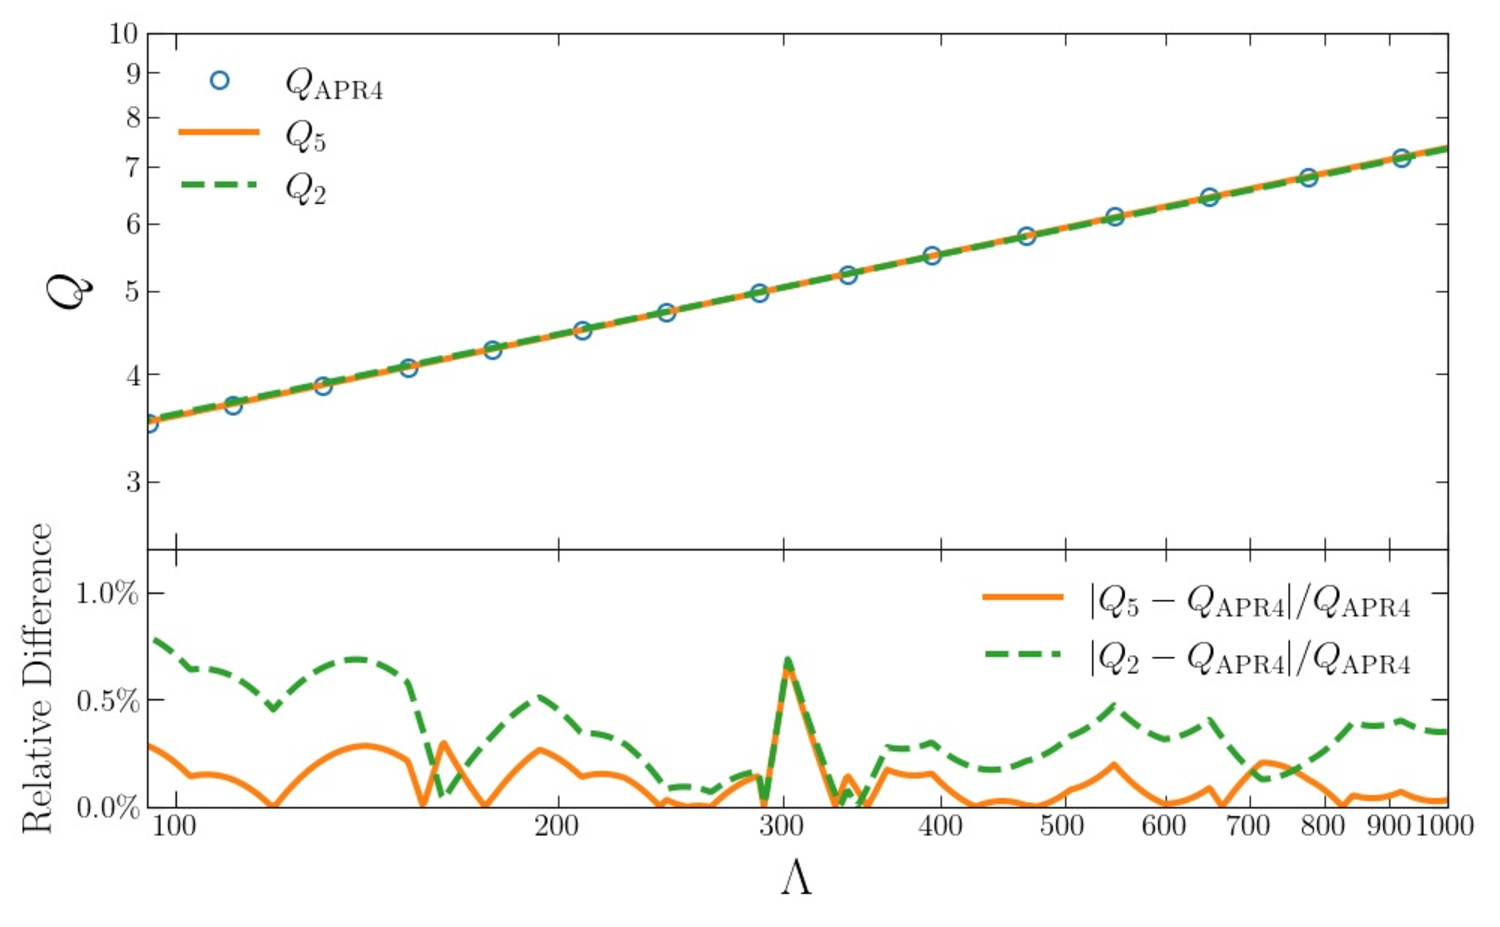
\includegraphics[width=0.8\textwidth]{2d-5d difference.pdf}% Here is how to import EPS art
\caption{\label{relative_difference} The upper panel shows the relation between $\Lambda$ and $Q$ for the Yagi-Yunes relation (eq.~\ref{5-d_Love_Q_eq}) and its linear fit (eq.~\ref{2-d_Love_Q_eq}). $\Lambda$ and $Q$ calculated assuming AP4 EOS are also plotted as a comparison ($Q_{\mathrm{AP4}}$). The lower panel shows the relative differences.}
\end{figure}

%=============================
\subsection{Principles}
\label{sec2_2}
%=============================

Hierarchical Bayesian inference is a framework that allows us to combine multiple observations to infer the hyper-parameters in a systematic way. In this framework, we want to find the posterior distribution of the hyper-parameters $p(\bm{H}|D)$. The data $D=\{d_1,...,d_n\}$ contains data streams $d_i$ of $n$ GW events from the detector network. Hyper-parameters and single-event parameters are unknown. We apply Bayes' theorem first to obtain the posterior of the hyper-parameters $\bm{H}$ and the waveform parameters $\{\bm{\theta}_1,...,\bm{\theta}_n\}$
\begin{equation}
\label{bayes2}
p(\bm{H},\bm{\theta}_1,...,\bm{\theta}_n|D)=\pi(\bm{H},\bm{\theta}_1,...,\bm{\theta}_n)\frac{p(D|\bm{H},\bm{\theta}_1,...,\bm{\theta}_n)}{p(D)}\,,
\end{equation}
where $\pi(\bm{H},\bm{\theta}_1,...,\bm{\theta}_n)$ is the prior probability density for the hyper-parameters and waveform parameters, $p(D|\bm{H},\bm{\theta}_1,...,\bm{\theta}_n)$ is the likelihood function, and $p(D)$ is the evidence which we do not need to calculate. To acquire the marginalized posterior for only hyper-parameters, we marginalize over the entire parameter space
\begin{equation}
\label{bayes1}
p(\bm{H}|D) = \int p(\bm{H},\bm{\theta}_1,...,\bm{\theta}_n|D) \text{d}\bm{\theta}_1...\text{d}\bm{\theta}_n\,,
\end{equation}

We first consider the priors. Assuming that the $n$ events are independent, the prior can be decomposed into parts of hyper-parameters and waveform parameters using the product rule of probability $p(A,B)=p(A)p(B|A)$
\begin{equation}
\label{bayes3}
\pi(\bm{H},\bm{\theta}_1,...,\bm{\theta}_n) = \pi(\bm{H}) \prod_{i=1}^n \pi(\bm{\theta}_i|\bm{H})\,.
\end{equation}
We treat $\Lambda$ and $Q$ as independent variables. We divide the set of waveform parameters for each event $\bm{\theta}_i$ into three categories: the tidal deformability parameters $\bm{\Lambda}_i=\{\Lambda_{1i},\Lambda_{2i}\}$, the quadrupole moment parameters $\bm{Q}_i=\{Q_{1i},Q_{2i}\}$, and the nuisance parameters $\bm{\xi}_i$. We assume that the prior distributions for nuisance parameters, including the two mass parameters, are independent of $\bm{\Lambda}_i, \bm{Q}_i$ and $\bm{H}$, given that no particular EOS is chosen in the inference procedure. 

Note that we make no assumptions of EOS in the hierarchical Bayesian inference part and EOS does not emerge in the conditional probability functions, given that the Love-Q relation is EOS-insensitive. 

In this way, the conditional prior for the waveform parameters in eq.~(\ref{bayes3}) can be further decomposed with the product rule
\begin{equation}
\label{prior}
\pi(\bm{\theta}_i|\bm{H})=\pi(\bm{\Lambda}_i|\bm{H})\pi(\bm{Q}_i|\bm{\Lambda}_i,\bm{H})\times\pi(\bm{\xi}_i)\,.
\end{equation}

Analogously to the prior, we decompose the likelihood into a product of single-event likelihoods for $n$ independent BNS observations
\begin{subequations}
\begin{align}
p(D|\bm{H},\bm{\theta}_1,...,\bm{\theta}_n)=\prod_{i=1}^{n}p(\bm{d}_i|\bm{H},\bm{\theta}_i)=\prod_{i=1}^{n}p(\bm{d}_i|\bm{\theta}_i)\,,
\end{align}   
\end{subequations}
note that in the second line we have used the fact that the hyper-parameters do not enter the waveform thus the likelihood only depends on $\bm{\theta}_i$, i.e. $p(\bm{d}_i|\bm{H},\bm{\theta}_i)=p(\bm{d}_i|\bm{\theta}_i)$.


Based on the derivation above, now the marginalized posterior distribution (eq.~(\ref{bayes1})) is
\begin{equation}
\label{hierarchical bayes}
\begin{aligned}
p(\bm{H}|D)&=\frac{1}{p(D)}\pi(\bm{H})\int \text{d}\bm{\theta}_1...\text{d}\bm{\theta}_n \prod_{i=1}^n \left[\pi(\bm{\Lambda}_i|\bm{H})\pi(\bm{Q}_i|\bm{\Lambda}_i,\bm{H})\pi(\bm{\xi}_i)p(\bm{d}_i|\bm{\theta}_i)\right] \\
&=\frac{1}{p(D)} \pi(\bm{H}) \prod_{i=1}^n
\int \text{d}\bm{\Lambda}_i\text{d}\bm{Q}_i\pi(\bm{\Lambda}_i|\bm{H})\delta(\bm{Q}_i-\bm{f}(\bm{\Lambda}_i;\bm{H})) \int \text{d}\bm{\xi}_i \pi(\bm{\xi}_i)p(\bm{d}_i|\bm{\theta}_i)\\
&=\frac{1}{p(D)} \pi(\bm{H}) \prod_{i=1}^n
\int \text{d}\bm{\Lambda}_i\pi(\bm{\Lambda}_i|\bm{H})L_i\left(\bm{\Lambda}_i,\bm{f}(\bm{\Lambda}_i;\bm{H})\right)\,,
\end{aligned}
\end{equation}
where the quasi-likelihood function for $\bm{\Lambda}_i,\bm{Q}_i$ is
\begin{equation}
\label{quasi-likelihood}
    L_i(\bm{\Lambda}_i,\bm{Q}_i)=\int \text{d}\bm{\xi}_i \pi(\bm{\xi}_i)p(\bm{d}_i|\bm{\theta}_i)\,.
\end{equation}

In the hierarchical Bayesian framework, the quasi-likelihoods can be computed independently on $\bm{H}$

%What we need to compute now are the quasi-likelihood functions (eq.~(\ref{quasi-likelihood})) for each GW event and then 
%substitute them into eqs.~(\ref{hierarchical bayes}). Since the hyper-parameters $\bm{H}$ do not appear in eq.~(\ref{quasi-likelihood}) 
%and $L_i(\bm{\Lambda}_i,\bm{Q}_i)$ only depend on the data and parameters of the $i\text{-th}$ event, we can perform a single-event Bayesian inference for each event 
%respectively to compute its quasi-likelihood function~\cite{Lackey:2014fwa, Thrane:2018qnx, Golomb:2021tll, Wang:2024xon}. 

For the $i\text{-th}$ event, we write down Bayes' theorem
\begin{equation}
\label{single bayes}
    p(\bm{\theta}_i|\bm{d}_i)\propto \pi(\bm{\theta}_i|\varnothing)p(\bm{d}_i|\bm{\theta}_i)\,,
\end{equation}
where $\pi(\bm{\theta}_i|\varnothing)$ is regarded as an auxilliary prior independent on $\bm{H}$. $p(\bm{d}_i|\bm{\theta}_i)$ is the single-event likelihood~\cite{Finn:1992wt} given by
\begin{equation}
p(\bm{d}_i|\bm{\theta}_i)\propto \mathrm{e}^{-\frac{1}{2}\langle d_i-h(\bm{\theta}_i),d_i-h(\bm{\theta}_i)\rangle}\,.
\end{equation}
$h(\bm{\theta}_i)$ is given by the waveform model we select. $\langle g, h\rangle$ is the inner product of $g(t)$ and $h(t)$ weighted by the power spectrum density (PSD) of $S_n(f)$ of the noise.
\begin{equation}
    \langle g, h\rangle:= 2\int_{-\infty}^{\infty}\frac{\tilde{g}(f)\tilde{h}^{*}(f)}{S_n(|f|)} \text{d}f\,,
\end{equation}
where $\tilde{g}(f)$ and $\tilde{h}(f)$ are the Fourier transforms of $g(t)$ and $h(t)$.

Rearranging terms of eq.~(\ref{single bayes}) and substituting it into eq.~(\ref{quasi-likelihood}), we obtain
\begin{equation}
\label{quasi-posterior}
\begin{aligned}
    L_i(\bm{\Lambda}_i,\bm{Q}_i) = \int \text{d}\bm{\xi}_i \pi(\bm{\xi}_i)p(\bm{d}_i|\bm{\theta}_i) \propto \int \text{d}\bm{\xi}_i \frac{\pi(\bm{\xi}_i)}{\pi(\bm{\theta}_i|\varnothing)}p(\bm{\theta}_i|\bm{d}_i)\,,
\end{aligned}  
\end{equation}
which allows us to construct the quasi-likelihood functions with posteriors given by single-event inferences. $p(\bm{\theta}_i|\bm{d}_i)$ can be obtained before the inference of $\bm{H}$ according to eq.~(\ref{single bayes}). 
From which we can see that the single-event parameters and hyper-parameters are inferred hierarchically. 
eq.~() and. In particular, as long as we choose flat priors for tidal and quadrupole moment parameters, the quasi-likelihood function is proportional to the marginalized posterior for every single event. 


%=============================
\section{Simulation}
\label{sec3}
%=============================

%=============================
\subsection{Waveform, Population and Detectors}
\label{sec3_1}
%=============================

For our simulation, we adopt the {\sc imrphenomxas\_nrtidalv3} waveform model~\cite{Abac:2023ujg}, which is an aligned spin waveform model and includes tidal amplitude corrections as well as spin-induced quadrupole moment terms up to 3.5PN. The parameter set is composed of the binary masses $m_1$ and $m_2$, the dimensionless tidal deformabilities $\Lambda_1$ and $\Lambda_2$ and spin-induced quadrupole moments $Q_1$ and $Q_2$ of each component, the dimensionless spin aligned with the direction of the orbital angular momentum $\chi_i$, the luminosity distance $D_L$, the merge time $t_c$, the right ascension $\alpha$ and declination $\delta$, the inclination angle $\iota$, the GW polarization angle $\psi$ and the phase of coalescence $\phi_c$. We denote the entire parameter set as a vector $\bm{\theta}$, i.e.
\begin{equation}
\label{parameter set}
\bm{\theta} = \{m_1,m_2,\Lambda_1,\Lambda_2,Q_1,Q_2,\chi_1,\chi_2,D_L,t_c,\alpha,\delta,\iota,\psi,\phi_c\}\,.
\end{equation}

We adopt the BNS mass population model proposed by Farrow~et~al.~\cite{Farrow:2019xnc}. According to their spin magnitude, the model divides BNS into a recycled star and a nonrecycled (\emph{slow}) one, for which the masses are labeled $m_r$ and $m_s$, respectively. The distribution of $m_r$ has two Gaussian components while $m_s$ follow a Uniform distribution,
\begin{subequations}
\label{mass population}
\begin{equation}
    P(m_r) = \alpha \mathcal{N}(\mu_1, \sigma_1) + (1-\alpha) \mathcal{N}(\mu_2, \sigma_2)\,,
\end{equation}
\begin{equation}
    P(m_s) = \mathcal{U}(m_s^l, m_s^u)\,,
\end{equation}
\end{subequations}
where $\alpha=0.68$, $\mu_1=1.34\mathrm{M}_{\odot}$, $\sigma_1=0.02\mathrm{M}_{\odot}$, $\mu_2=1.47\mathrm{M}_{\odot}$, $\sigma_2=0.15\mathrm{M}_{\odot}$ and $m_s^l=1.14\mathrm{M}_{\odot}$, $m_s^u=1.46\mathrm{M}_{\odot}$. When generating simulation GW signals, for each event we just select the larger one of $m_r$ and $m_s$ as the primary mass $m_1$ and the other as the secondary mass $m_2$, since we always demand $m_1 \geq m_2$.

The tidal deformability and quadrupole moments of the binary are calculated from the stellar mass assuming the AP4 EOS, which is a soft EOS consistent with the LIGO-Virgo tidal measurements~\cite{LIGOScientific:2017vwq, LIGOScientific:2018cki, LIGOScientific:2018hze}. Refs.~\cite{Yagi:2013awa, Atta:2024ckt} demonstrates in detail how to derive tidal deformability $\Lambda_i$ and quadrupole moment $Q_i$ given the mass $m_i$ and the EOS. For the dimensionless spin component $\chi_r$ of recycled stars, we adopt a uniform distribution $\mathcal{U}(-0.5,0.5)$, 
while in the case of slow stars, the spin $\chi_s$ is drawn from $\mathcal{U}(-0.1,0.1)$.

Using the cosmological parameters provided by the Planck Collaboration~\cite{Planck:2018vyg}, we simulate 1000 GW sources distributed uniformly in co-moving volume from 15Mpc to 150Mpc~\cite{Fishbach:2018edt, KAGRA:2021duu}, with isotropic sky locations and orientations. This corresponds to the observed local 
%########
merger rate $R=320_{-270}^{+490}\,\mathrm{Gpc}^{-3}\mathrm{yr}^{-1}$ from current GW detections~\cite{LIGOScientific:2020aai}. 
%########
Without loss of generality, all these GW events are injected with an arbitrary coalescence time $t_c=0$.

We select a ground-based network consisting of two CE detectors and one ET detector. We use the noise curves of the CE and ET detectors with the CE-2~\cite{Reitze:2019iox, Reitze:2019dyk} and ET-D~\cite{Punturo:2010zz, Hild:2010id, Sathyaprakash:2012jk} configurations respectively. The two CE detectors are positioned at the current sites of the two LIGO detectors, while the ET detector is set at the current location of the Virgo detector with a triangular shape. 

%=============================
\subsection{Implementation}
\label{sec3_2}
%=============================

The evaluation of the marginalized posterior for hyper-parameters can be divided into two steps, according to the discussion in section~\ref{sec2_2}. We firstly perform Bayesian inference for each event. The quasi-likelihood (eq.~(\ref{quasi-posterior})) can be obtain through a density estimation method introduced by ref.~\cite{Talbot:2020oeu}; 
then we substitute the quasi-likelihoods into eq.~(\ref{hierarchical bayes}) and finish the integral as the likelihood of the hyper-parameter inference. Secondly, we perform another sampling procedure to finally obtain the posterior samples of hyper-parameters with flat priors. 

In the first step, when conducting single-event Bayesian inference, we choose $\mathcal{M}$ and $\eta$ as mass parameters. In this way, the parameter set of single-event Bayesian inference becomes $\bm{\theta} = \{\mathcal{M},\eta,\Lambda_1,\Lambda_2,Q_1,Q_2,\chi_1,\chi_2,D_L,t_c,\alpha,\delta,\iota,\psi,\phi_c\}$. The priors of $\mathcal{M},\eta,\chi_1,\chi_2,t_c,\phi_c$ are uniform, while the prior of $D_L$ is uniform in the co-moving volume and source frame time. We set isotropic priors for the angle variables $\alpha,\delta,\iota,\psi$. For tidal and quadrupole moment parameters, we treat $\Lambda_s$ and $Q_s$ of the slow binary component as nuisance parameters, considering that the spin-induced quadrupole moment is poorly estimated with low spin~\cite{Yagi:2013awa}. And we select uniform priors for $\Lambda_1,\Lambda_2$ and $Q_1,Q_2$ so that eq.~(\ref{quasi-posterior}) can be further simplified as
\begin{equation}
    \label{quasi-marginalized}
    \begin{aligned}
        L_i(\Lambda_{ri},Q_{ri}) \propto \int \text{d}\bm{\xi}_i \frac{\pi(\bm{\xi}_i)}{\pi(\bm{\theta}_i|\varnothing)}p(\bm{\theta}_i|\bm{d}_i) \propto \int \text{d}\bm{\xi}_i p(\bm{\theta}_i|\bm{d}_i)\propto p(\Lambda_{ri},Q_{ri}|\bm{d}_i)\,,
    \end{aligned}  
\end{equation}
where $\Lambda_{ri}$ and $Q_{ri}$ are the tidal deformability and quadrupole moment of the recycled binary component of the $i$-th event, respectively. Eq.~(\ref{quasi-marginalized}) indicates that the quasi-likelihood is proportional to the marginalized posterior $p(\Lambda_{ri},Q_{ri}|\bm{d}_i)$, revealing that we can directly construct the quasi-likelihood from posterior samples.

After sampling, we obtain the quasi-likelihood of each event from $\Lambda_r$ and $Q_r$ samples. To complete the integral in eq.~(\ref{hierarchical bayes}), we must create a functional form for each quasi-likelihood using the posterior samples. Following Golomb and Talbot~\cite{Golomb:2021tll}, we adopt the Gaussian mixture model (GMM) method developed by Ref.~\cite{Talbot:2020oeu} as the density estimation method to obtain the quasi-likelihood with eq.~(\ref{quasi-likelihood}). Substitute the results of density estimation into eq.~(\ref{hierarchical bayes}), and then the likelihood function of the hyper-parameter estimation can be constructed.

In the second step, we sample the integrand of eq.~(\ref{hierarchical bayes}) with Bayesian inference. For hyper-parameters $\pi(\bm{H})$, we use uniform priors with the boundaries listed in Table~\ref{prior_table} and for the prior $\pi(\bm{\Lambda}_i|\bm{H})$, we use the uniform distribution $\mathcal{U}(10,2000)$. For Bayesian inference in both steps, posterior samples are generated with {\sc NESSAI}~\cite{Skilling:2004pqw, Skilling:2006gxv, michael_j_williams_2025_14627250, PhysRevD.103.103006, Williams:2023ppp} of the {\sc BILBY}~\cite{Ashton:2018jfp} package. We simulate 1000 GW events as described in section~\ref{sec3_1}. 

% SNR挑选和自旋挑选分开
Ref.~\cite{Lackey:2014fwa} found that the overwhelming majority of the information for population properties comes from the evnets with the highest SNRs and ref.~\cite{Yagi:2013awa} concluded that the spin-induced quadrupole moment is poorly estimated with a low spin. Considering these findings, we only pick some of the simulated GW sources and leave the full-population study for future work. In practice, we first draw 100 sources with the highest SNRs; then among these 100 sources we further select 20 sources whose recycled components rotate the fastest (i.e. with the largest $|\chi_{ri}|$). 

\begin{table}[htbp]
    \centering
    \sisetup{
        table-align-text-post = false, 
        separate-uncertainty = true 
    }
    \caption{\label{prior_table}The best fit values of Yagi-Yunes relation and the priors of the hyper-parameters in different polynomial fitting models with $i=2, 3, 4, 5$ parameters for the Bayesian inference. Regarded as reference values}
    \begin{tabular}{
        l
        S[table-format=-1.4]
        S[table-format=1.5]
        S[table-format=1.3e-1]
        S[table-format=-1.3e-1]
        S[table-format=1.3e-1]
    }
        \toprule
        \multicolumn{6}{c}{Best fit values} \\
        %\cmidrule(l){2-6}
        $i$ & {$a_i$} & {$b_i$} & {$c_i$} & {$d_i$} & {$e_i$} \\
        \midrule

        5 \, &  0.1940 & 0.0916 & 4.812e-2 & -4.283e-3 & 1.245e-4 \\
        4 \, &  0.1290 & 0.1480  & 3.021e-2 & -1.817e-3 & {/}      \\
        3 \, & -0.0709 & 0.2775  & 3.220e-3 & {/}       & {/}      \\
        2 \, & -0.1457 & 0.3094  & {/}      & {/}       & {/}      \\
        
        \midrule

        \multicolumn{6}{c}{Priors} \\
        %\cmidrule(l){2-6}
        $i$ & {$a_i$} & {$b_i$} & {$c_i$} & {$d_i$} & {$e_i$} \\
        \midrule

        5 \, & {$\mathcal{U}(-5.0, 5.0)$} & {$\mathcal{U}(-1.0, 1.0)$} & {$\mathcal{U}(-0.5, 0.5)$} & {$\mathcal{U}(-0.1, 0.1)$} & {$\mathcal{U}(-0.01, 0.01)$} \\
        4 \, & {$\mathcal{U}(-5.0, 5.0)$} & {$\mathcal{U}(-1.0, 1.0)$} & {$\mathcal{U}(-0.5, 0.5)$} & {$\mathcal{U}(-0.1, 0.1)$} & {/}                         \\
        3 \, & {$\mathcal{U}(-5.0, 5.0)$} & {$\mathcal{U}(-1.0, 1.0)$} & {$\mathcal{U}(-0.5, 0.5)$} & {/}                       & {/}                         \\
        2 \, & {$\mathcal{U}(-5.0, 5.0)$} & {$\mathcal{U}(-1.0, 1.0)$} & {/}                       & {/}                       & {/}                         \\
        \bottomrule
    \end{tabular}
\end{table}


%=============================
\section{Results and Discussions}
\label{sec4}
%=============================

%=============================
\subsection{Linear Fitting Model}
\label{sec4_1}
%=============================

\begin{figure}
    \centering
    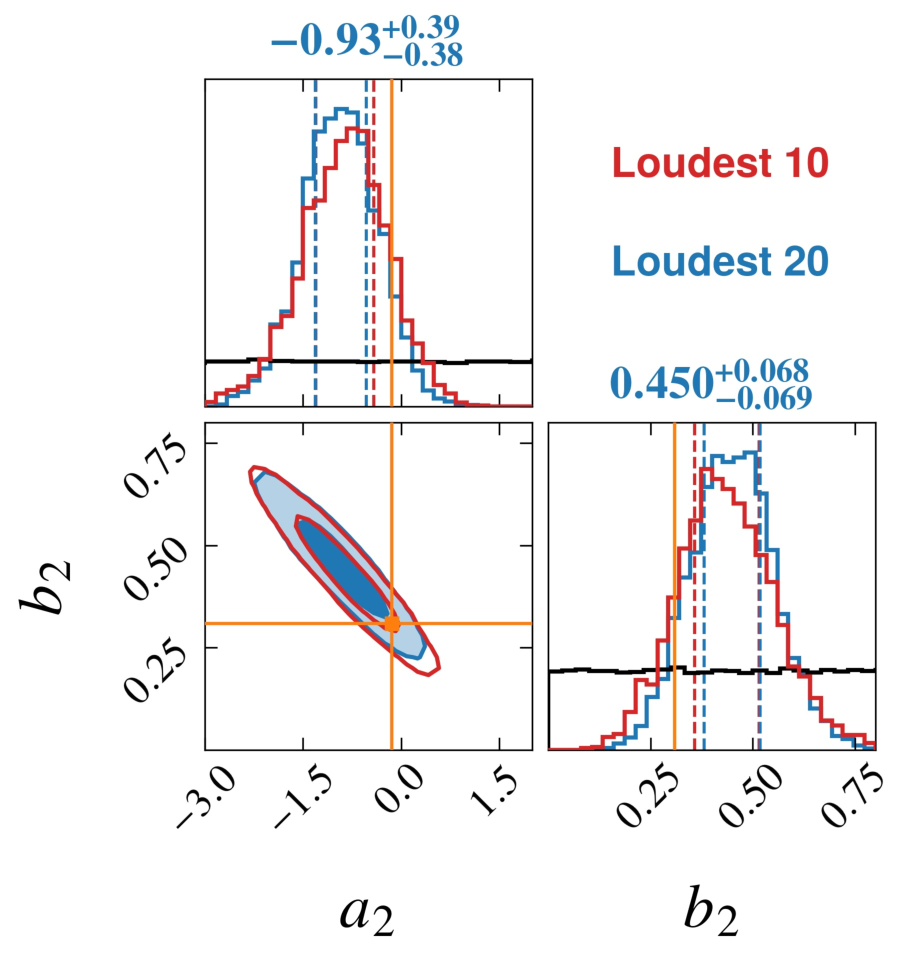
\includegraphics[width=0.5\linewidth]{comparison_corner_plot.pdf}
    \caption{Posterior distributions of the hyper-parameters in the linear fitting case. The contours refer to 50\% and 90\% credible regions for both inferences based on the loudest 10 and 20 events. The numbers above the histograms stand for the median and the central 50\% credible interval of each marginalized distribution in the 20 event inference. The orange lines represent the best fit values of the parameters in Table.~\ref{prior_table}. The priors are also drawn in black for the histograms on the diagonal.}
    \label{corner2-d}
\end{figure}

\begin{figure}
\centering
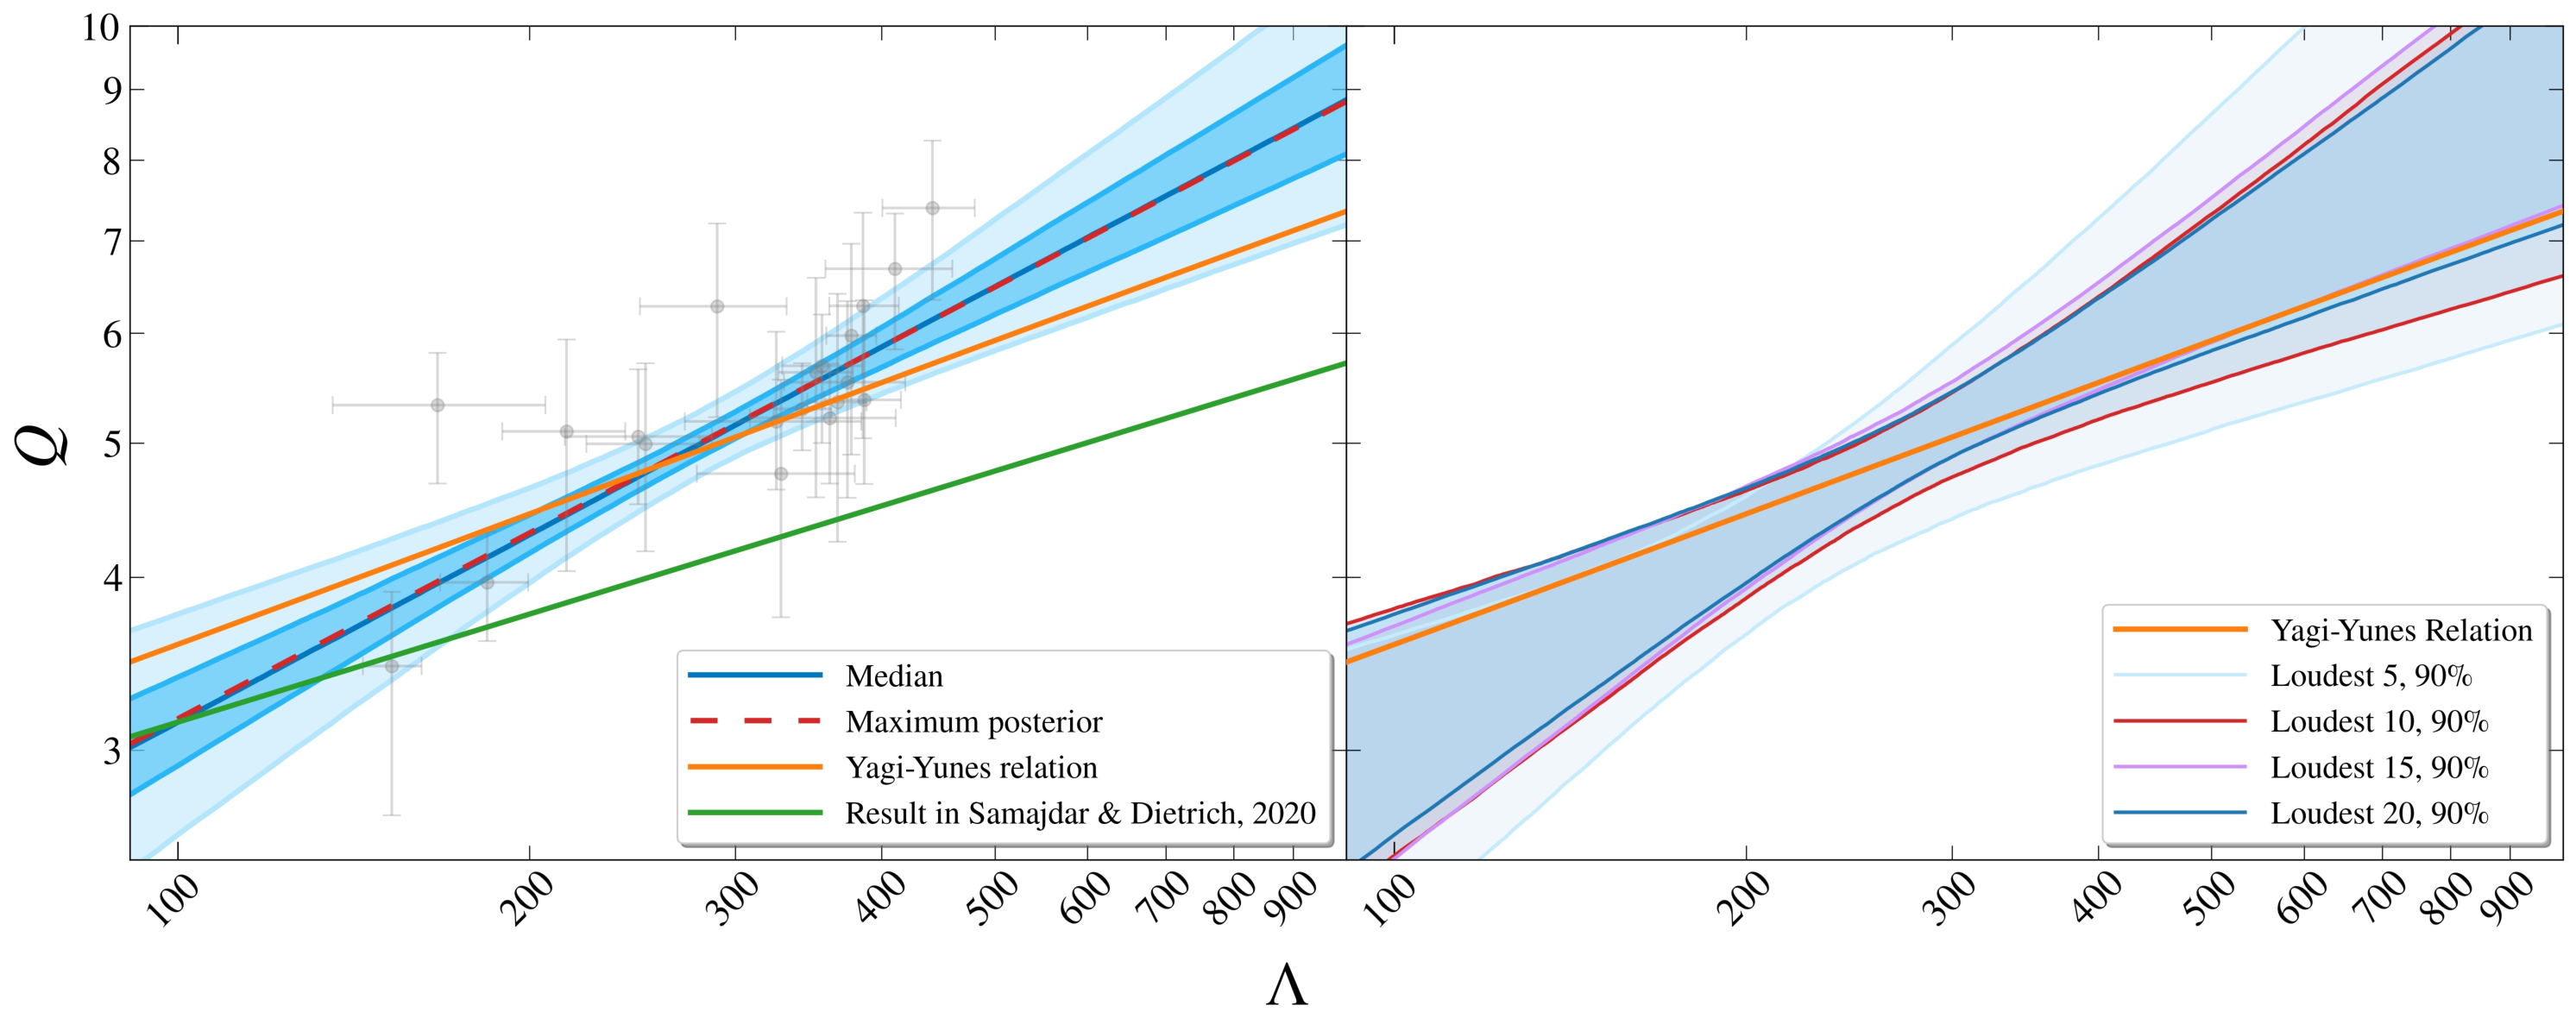
\includegraphics[width=\textwidth]{hierarchical_results_AP4_2d.pdf}
    \caption{Results of the hierarchical Bayesian inference for linear Love-Q relation. In the left panel, the Love-Q relation is inferred based on 20 simulated GW events. The gray error bars demonstrate the $1\sigma$ credible interval of $\Lambda$ and $Q$. The orange solid line represents the Yagi-Yunes Love-Q relation and the green solid line refs to the result given by Samajdar \& Dietrich, 2020~\cite{Samajdar:2020xrd}. The blue regions from dark to light represent the $50\%$ and $90\%$ credible intervals of $Q$. The blue solid line and the red dashed line are the median and peak of the distribution of $Q$ with certain $\Lambda$. In the right panel, contours correspond to $90\%$ credible intervals for the inference result based on the loudest 5, 10, 15, 20 events, respectively.
    \label{2-d_Love_Q}}
\end{figure}

Based on the methods discussed above, we perform the hierarchical Bayesian inference for linear Love-Q relations. Following Ref.~\cite{Lackey:2014fwa}, we show how the results depend on the number of events to verify if the major information for Love-Q relation is provided by sources with the highest SNR (loudest). The posterior distributions for the hyper-parameters of 10 event inference and 20 event inference are both shown in figure.~\ref{corner2-d} as a comparison. For the joint distribution in the lower left corner, we find that the credible regions of the two inferences are quite similar, and the best fit values listed in Table.~\ref{prior_table} are close to the edge of the 50\% credible regions in the joint distribution. Moreover, in both cases, correlation exists between the two hyper-parameters. 

%####################
In the diagonal corners, the peak values of the marginalized distributions for the two cases are also close to each other, indicating the dominance of events with higher SNR. An increase in the number of events just slightly narrows the peak width of the marginalized posteriors, and accordingly the 50\% credible region shrinks in the loudest 20 events case. 
%####################

In the left panel of figure.~\ref{2-d_Love_Q}, we plot the linear Love-Q relation according to the posterior samples. For a certain $\Lambda$, every sample point of hyper-parameters corresponds to a $Q$ value. With $\Lambda$ fixed, we find the $50\%$ and $90\%$ credible intervals of $Q$, and for continuously variable $\Lambda$, the intervals combine to form a region. As we can see, the Yagi-Yunes Love-Q relation is almost covered by the $90\%$ region. The credible intervals are wide at both ends and narrow in the middle, as most of the events concentrate in the $\Lambda \sim 400$ region. In the right panel, we compare the credible regions for inferences using the loudest 5, 10, 15 and 20 events. 
The $90\%$ regions for the latter three cases almost overlap each other. This means that the loudest 10 events dominate the results, and thus including much quieter events will not significantly improve the results.

%=============================
\subsection{Quartic Polynomial Fitting Model}
\label{sec4_2}
%=============================

\begin{figure}
\begin{minipage}[t]{0.49\textwidth}
\centering
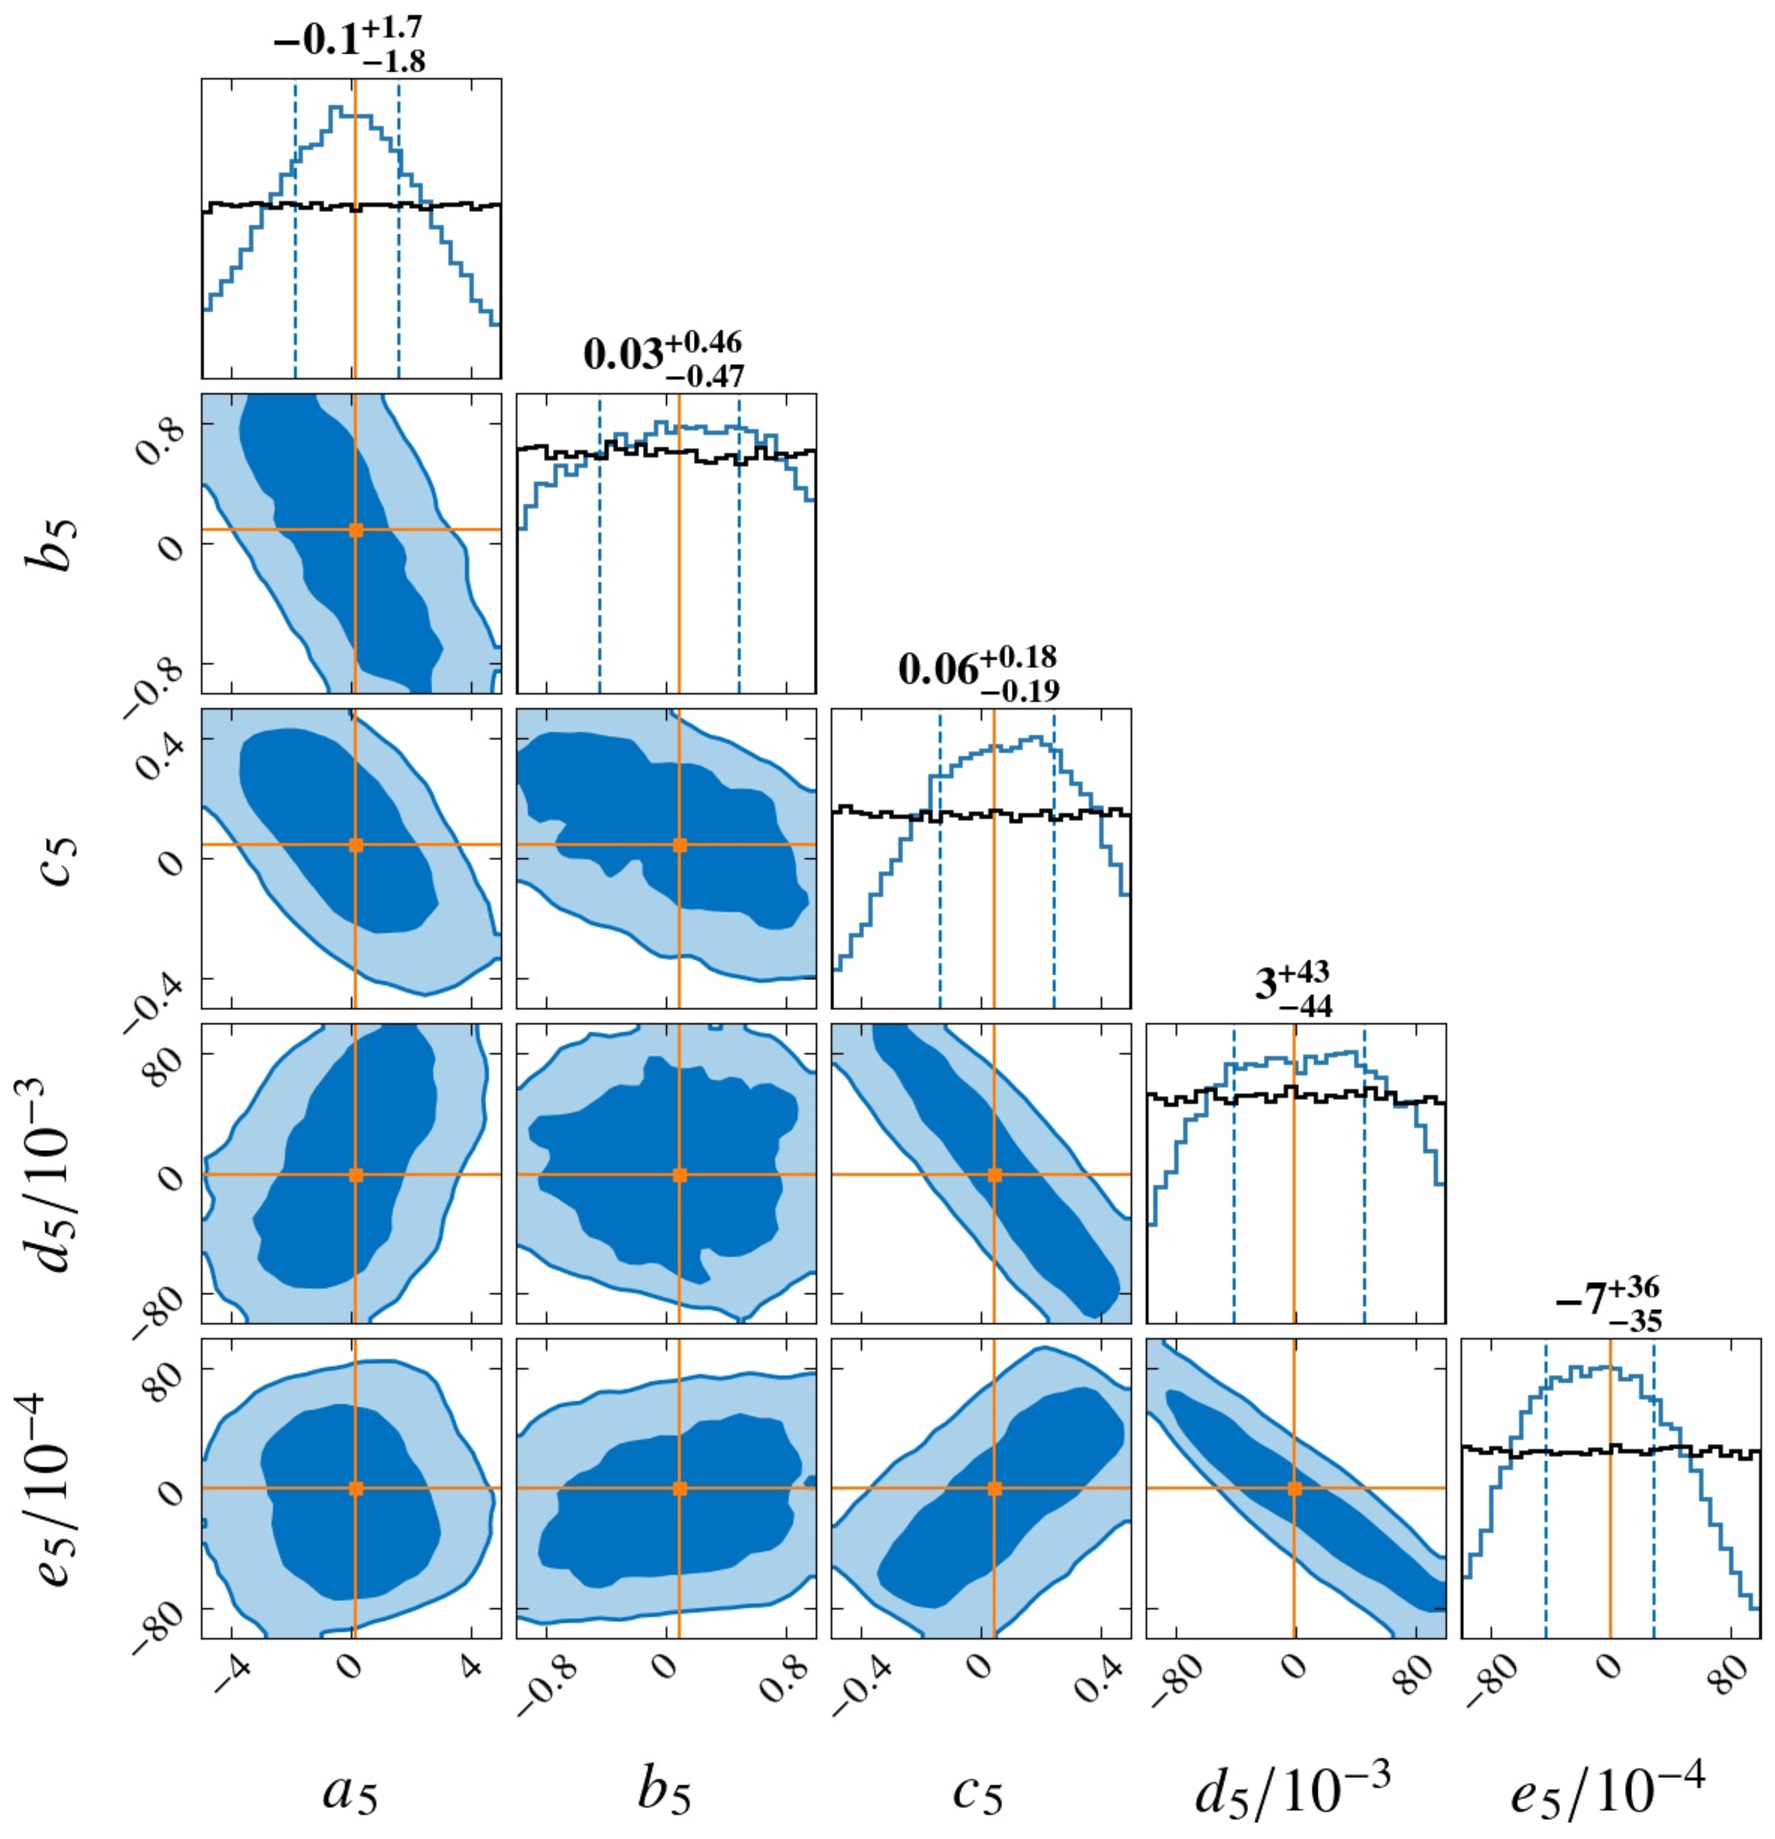
\includegraphics[width=0.8\linewidth]{Hyper_parameter_5d.pdf}% Here is how to import EPS art
\end{minipage}
\hfill
\begin{minipage}[t]{0.49\textwidth}
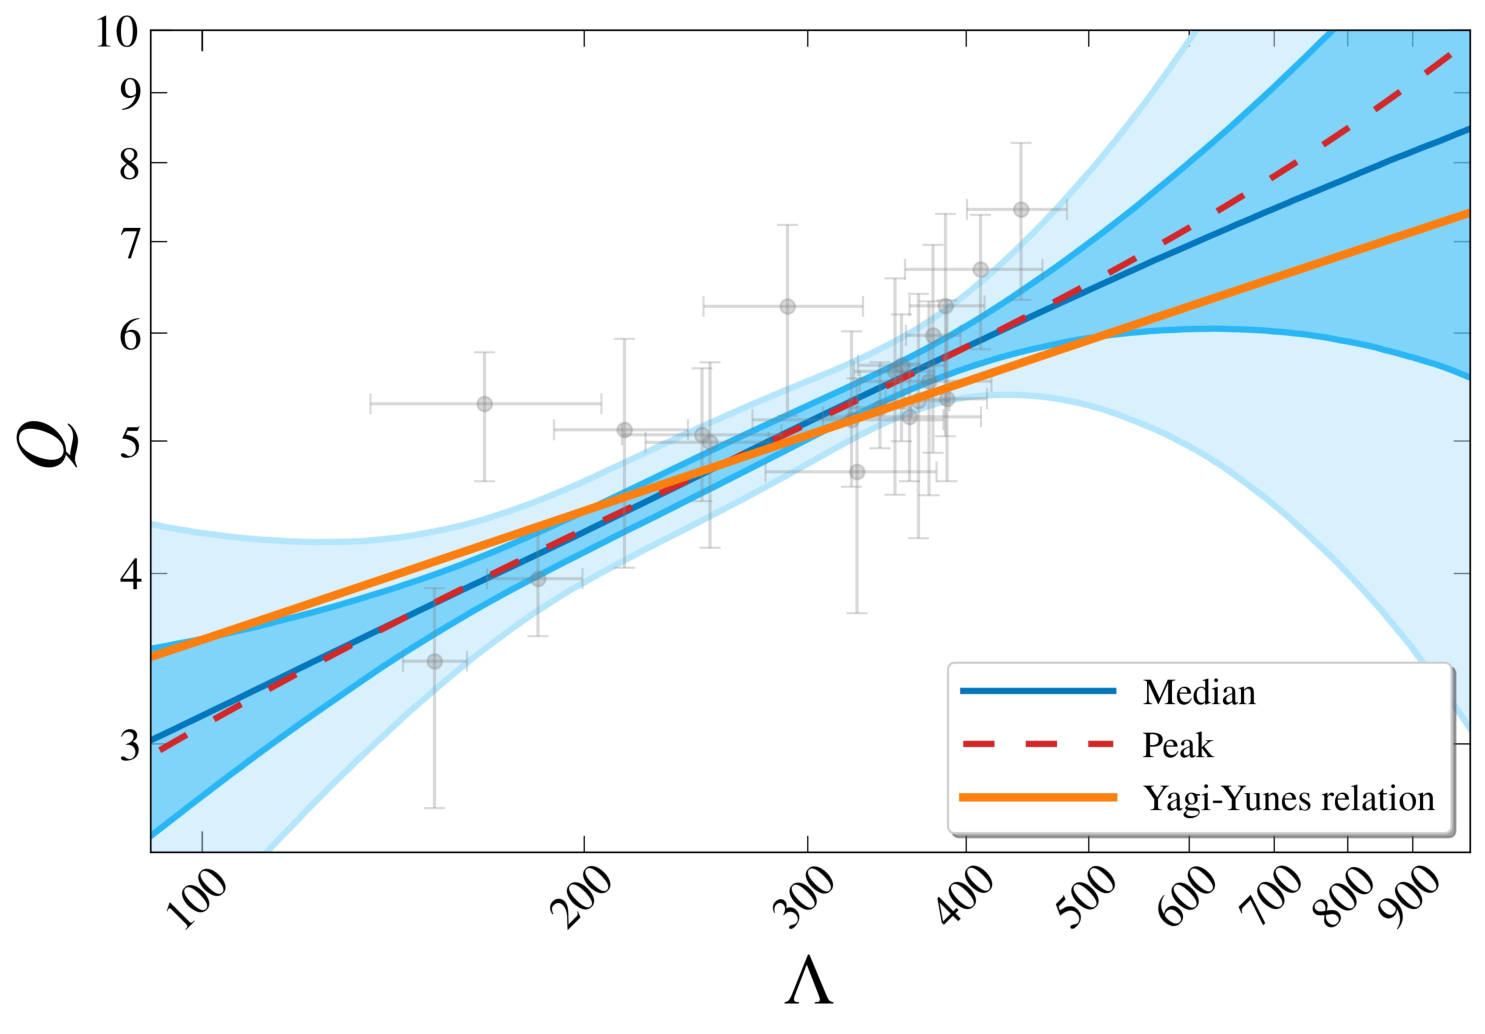
\includegraphics[width=\linewidth]{hierarchical_results_AP4_5d.pdf}
\end{minipage}
    \caption{\label{5-d_Love_Q} Left panel: posterior distribution of the hyper-parameters in the quartic polynomial fitting case. The inference is based on all of the 20 events. The orange lines represent the values in the Yagi-Yunes Love-Q relation. Right panel: similar to figure.~\ref{2-d_Love_Q}, but for the quartic polynomial fitting case. Still, the Yagi-Yunes Love-Q relation is included in the $90\%$ credible region.} 
\end{figure}

For the quartic polynomial fitting model, we parameterize the Love-Q relation by eq.~(\ref{5-d_Love_Q_eq}) and perform a hierarchical Bayesian inference for five hyper-parameter $\{a_5, b_5, c_5, d_5, e_5\}$. The left panel of figure~\ref{5-d_Love_Q} illustrates the posterior distributions of the hyper-parameters for this five-parameter model. Similarly to figure~\ref{corner2-d}, the priors and marginalized posteriors are plotted together in the diagonal histograms. 
The values taken in Yagi-Yunes Love-Q relation are closed to the marginalized distribution peaks, which become consistent with the maximum likelihood estimation given flat priors. Compared to the linear fitting case, these peaks are wider in the prior space and thus the credible regions in the two-parameter joint distributions become broader. 
This is reasonable since the increase in the degree of freedom makes it harder to constrain each parameter.

We summarize the quartic polynomial Love-Q relation constraining results in the right panel of figure~\ref{5-d_Love_Q} according to the posterior distributions. We mark the $50\%$ and $90\%$ credible intervals of $Q$ using the same method as the linear fitting model. Like in figure~\ref{2-d_Love_Q} for linear Love-Q relations, the Yagi-Yunes relation almost falls within the $90\%$ region. In addition, the widths of the $90\%$ regions with $\Lambda \sim 400$ in figure~\ref{5-d_Love_Q} and figure~\ref{2-d_Love_Q} are close, except for the wider end in five-parameter case when $\Lambda$ is large. This is understandable because $c_5, d_5$ and $e_5$ are much smaller than $a_5$ and $b_5$, making the $\ln^k\Lambda$ terms with $k\leq1$ dominate when $\Lambda$ is not large enough.

%=============================
\subsection{More Polynomial Fitting Models}
\label{sec4_3}
%=============================

\begin{figure}
    \begin{minipage}[t]{0.49\textwidth}
    \centering
    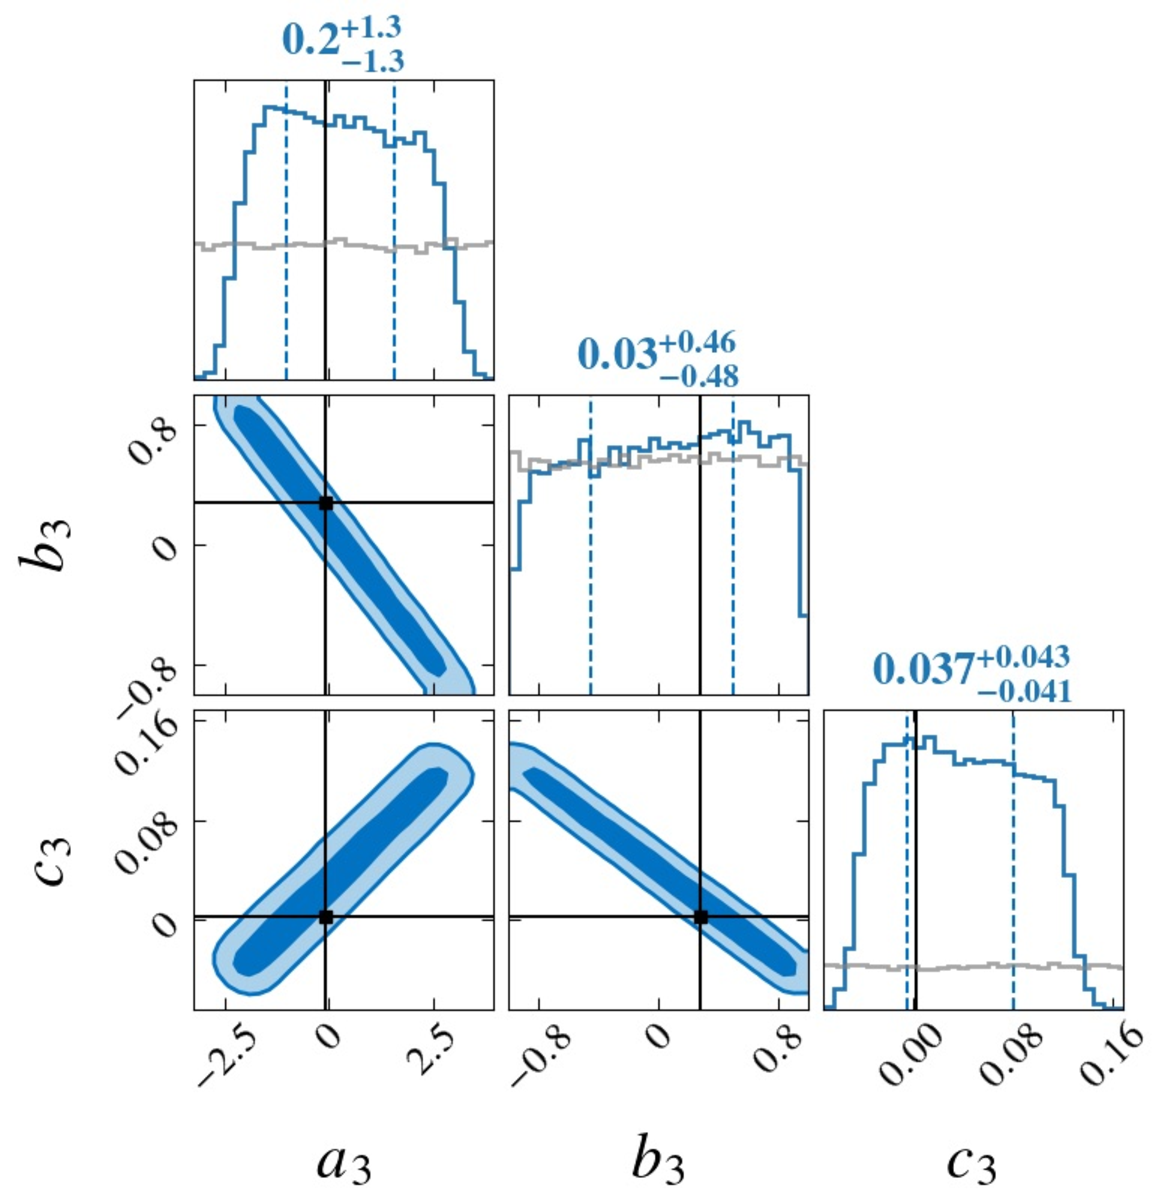
\includegraphics[width=0.8\linewidth]{Hyper_parameter_3d.pdf}% Here is how to import EPS art
    \end{minipage}
    \hfill
    \begin{minipage}[t]{0.49\textwidth}
    \centering
    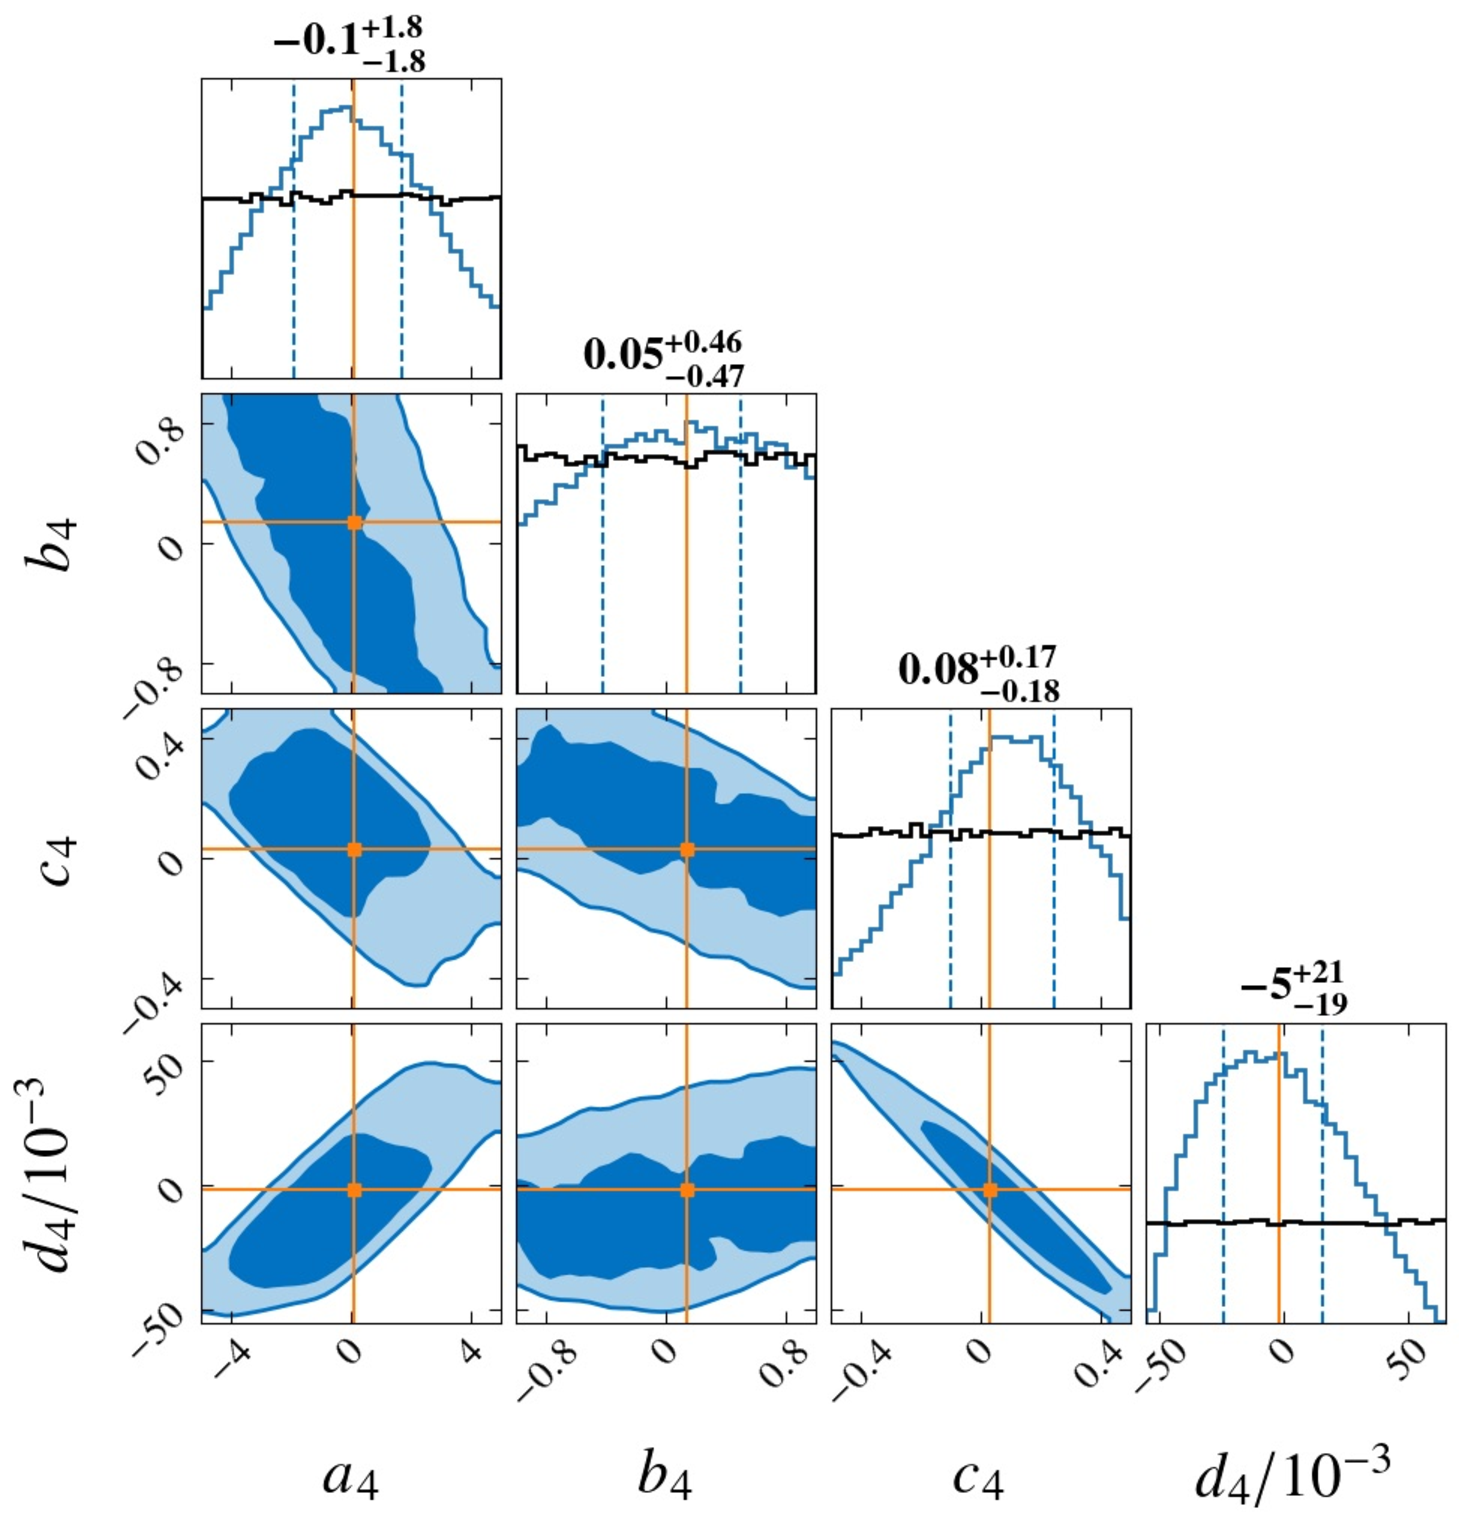
\includegraphics[width=0.8\linewidth]{Hyper_parameter_4d.pdf}
    \end{minipage}
    \vspace{3mm}
    \begin{minipage}[t]{\textwidth}
    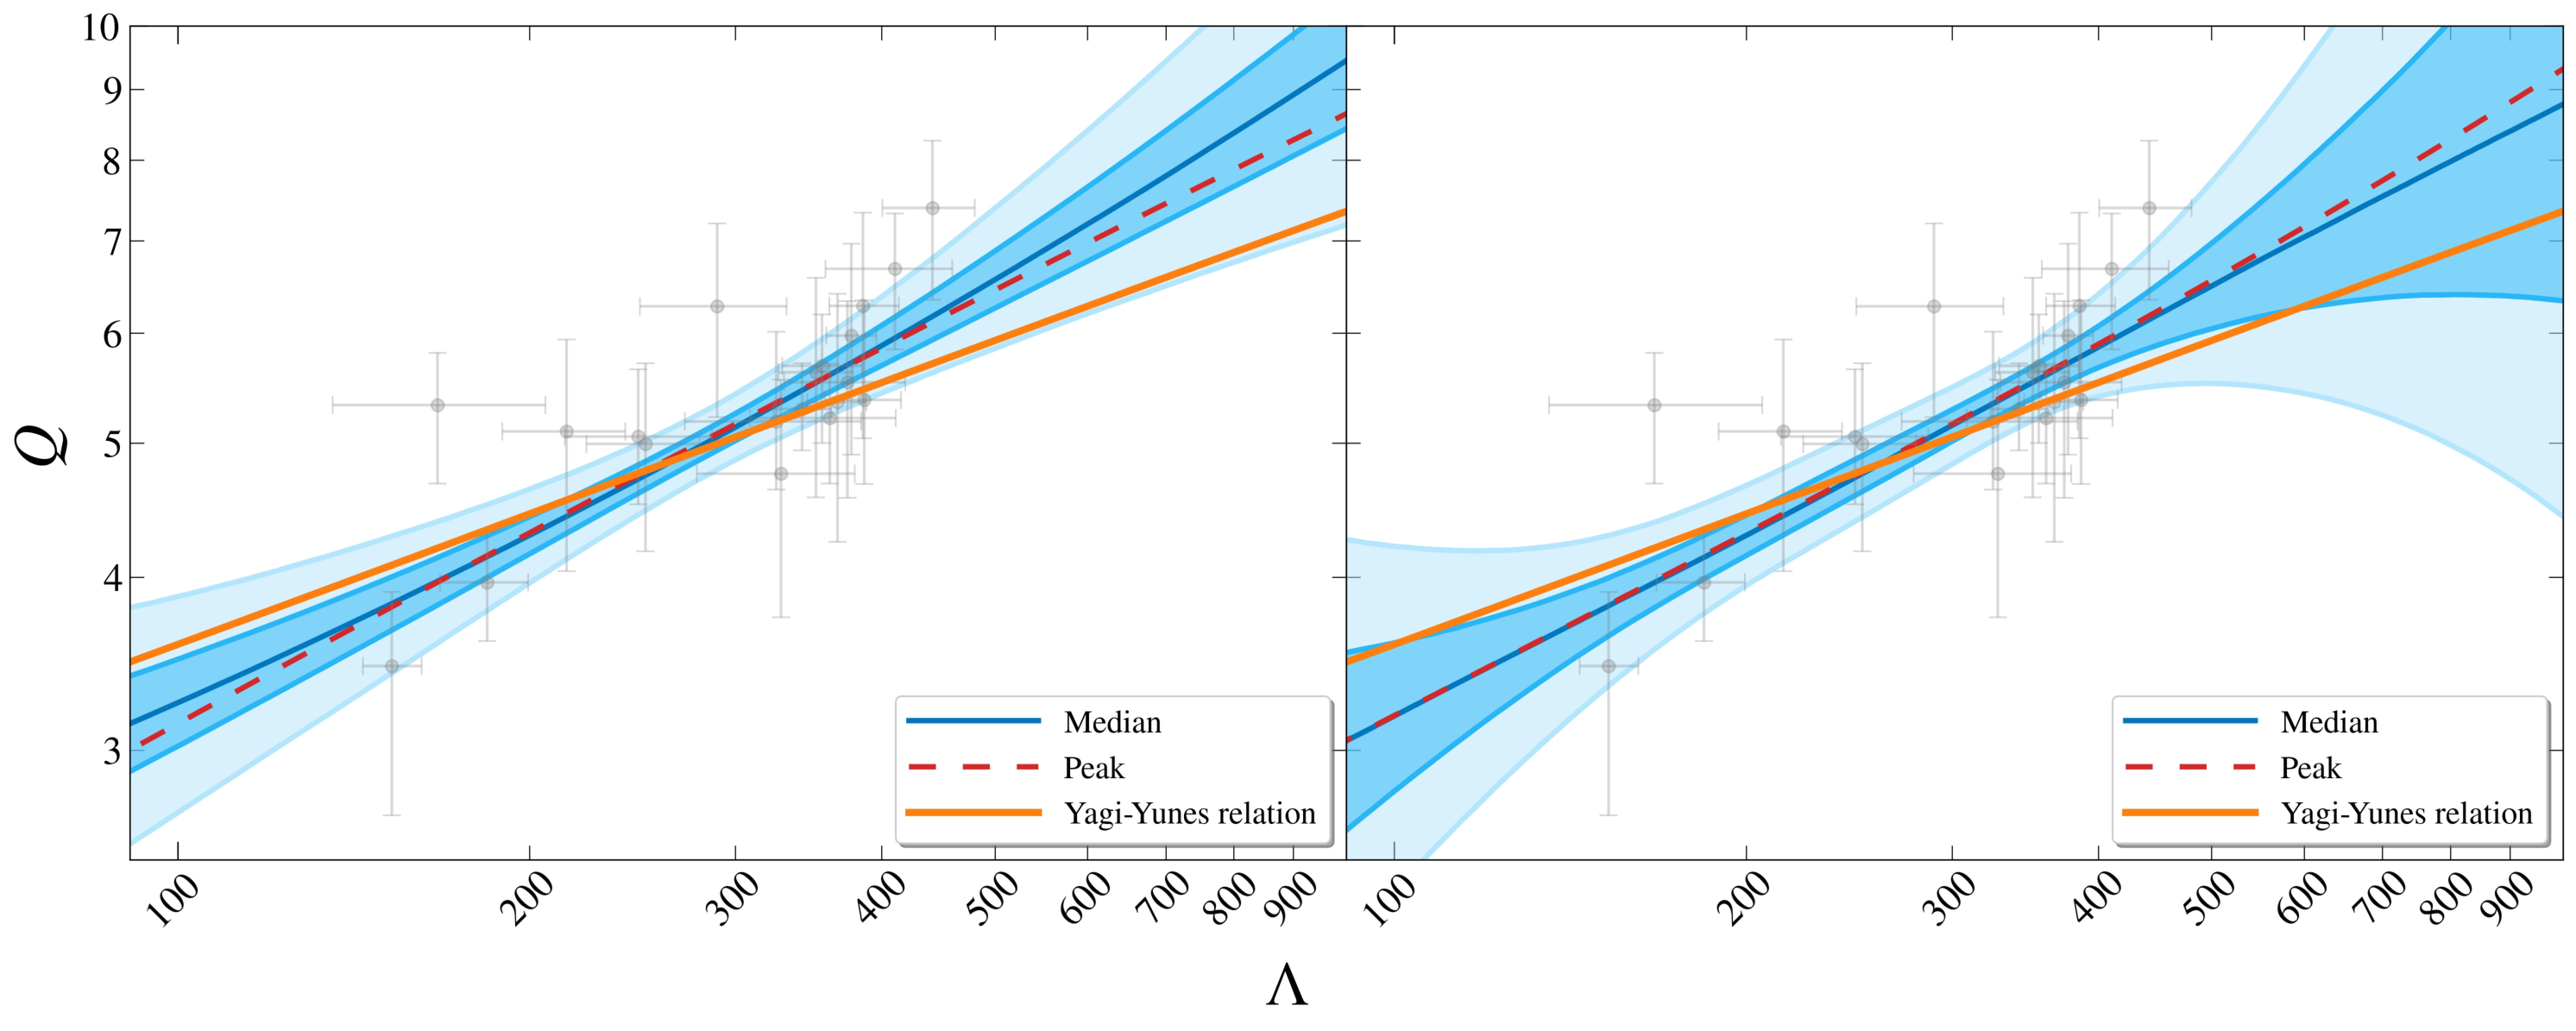
\includegraphics[width=\linewidth]{hierarchical_results_AP4_3d.pdf}% Here is how to import EPS art
    \end{minipage}
    \caption{\label{3-d_4-d_Love_Q} Results of quadratic and cubic polynomial fitting models. The 
    two upper panels demonstrate the posteriors of the hyper-parameters. And the best fit values (see table~\ref{prior_table}) 
    are marked in orange. The two bottom panels present the inference results in Love-Q plane, similar to 
    figure~\ref{2-d_Love_Q}.
    }
\end{figure}

We have mentioned in section~\ref{sec4_2} that it will be harder to constrain every hyper-parameter as the 
degree of freedom increases, thus we perform hyper-parameter inferences for quadratic and cubic polynomial (three-parameter and four-parameter) fitting models. Figure~\ref{3-d_4-d_Love_Q} demonstrates the posteriors and the corresponding Love-Q inference results for these two models. In the quadratic case, we find strong degeneracy among the three parameters. The marginalized posterior distributions of $a_3$ and $c_3$ have very wide and flat peaks, while $b_3$ is so poorly constrained that its posterior is similar to its prior. When it comes to the four-parameter inference results, degeneracy still emerges and again we find the marginalized posterior of one hyper-parameter $b_4$ resemble the prior. These results imply that for our simulation data size, a two-parameter linear fitting model is enough and the two fitting coefficients can be well constrained by our hierarchical Bayesian inference.

Same as before, we plot the constraint of Love-Q relation according to the posterior samples in the two lower panels 
of figure~\ref{3-d_4-d_Love_Q}. Like two-parameter and five-parameter results, the width of the $90\%$ region where most of the data points gather is insensitive to our parameterization of the Love-Q relation. We expect a better constraint to the both ends of the 90\% regions based on more GW events, which may contain more information for the behavior of the Love-Q relation with $\Lambda \sim 100$ or $\Lambda > 500$.

%=============================
\section{Testing Modified Gravity: Dynamical Chern-Simons Gravity}
\label{sec5}
%=============================

\begin{figure}[htbp]
    \centering
    \begin{minipage}{0.48\linewidth}
        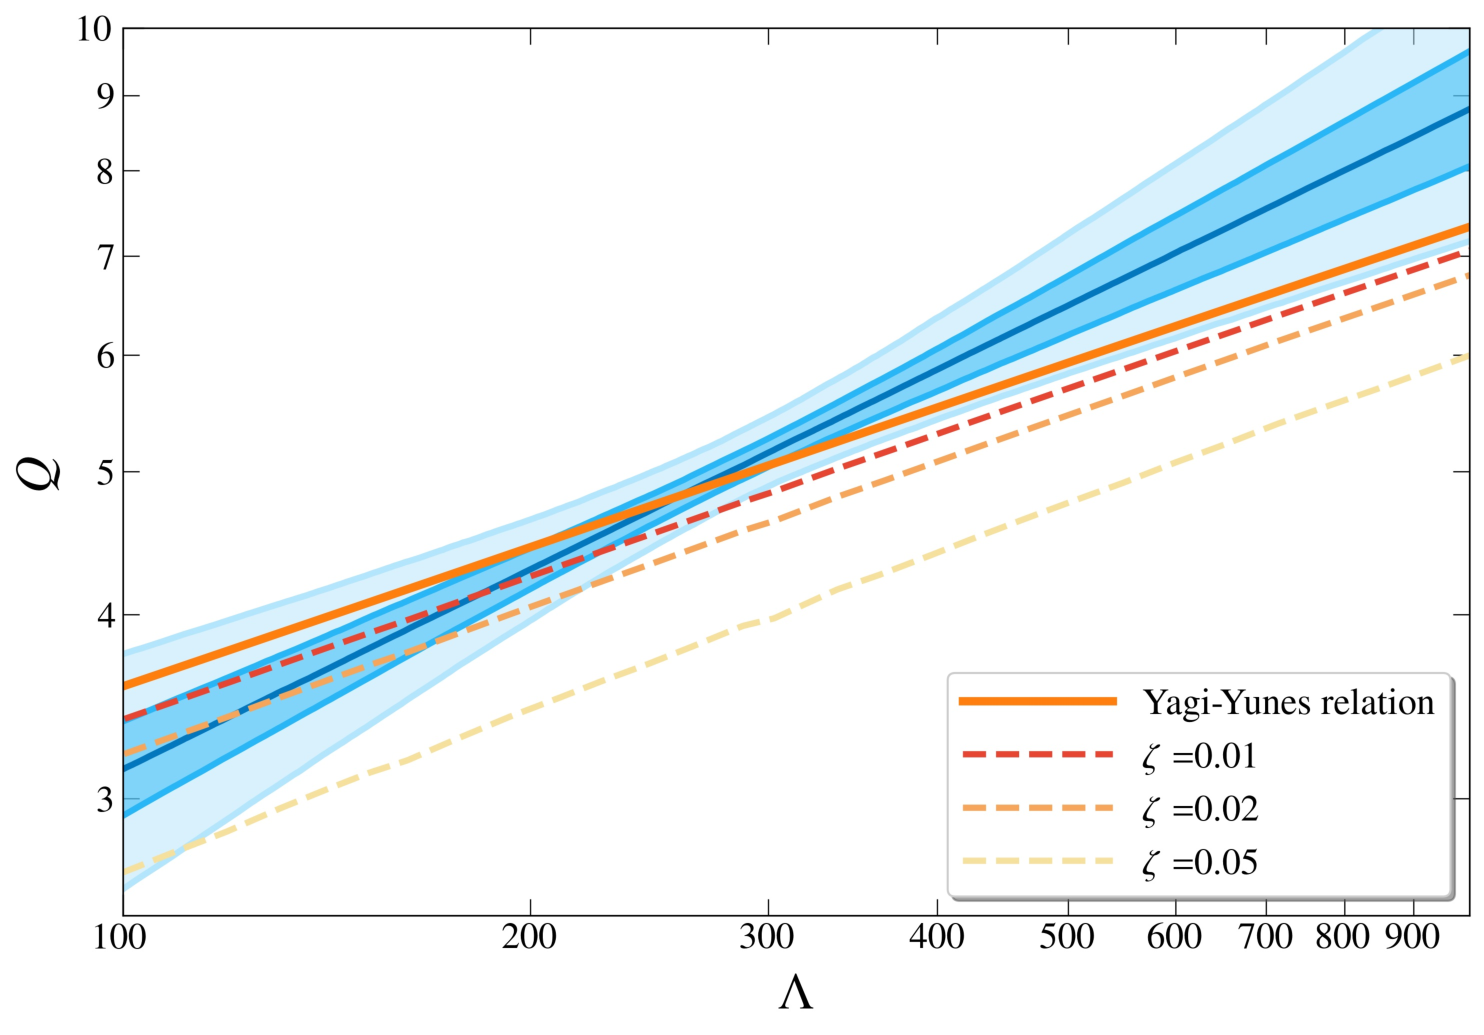
\includegraphics[width=\linewidth]{CS_zeta_AP4_2d.pdf}
    \end{minipage}
    \hfill
    \begin{minipage}{0.48\linewidth}
        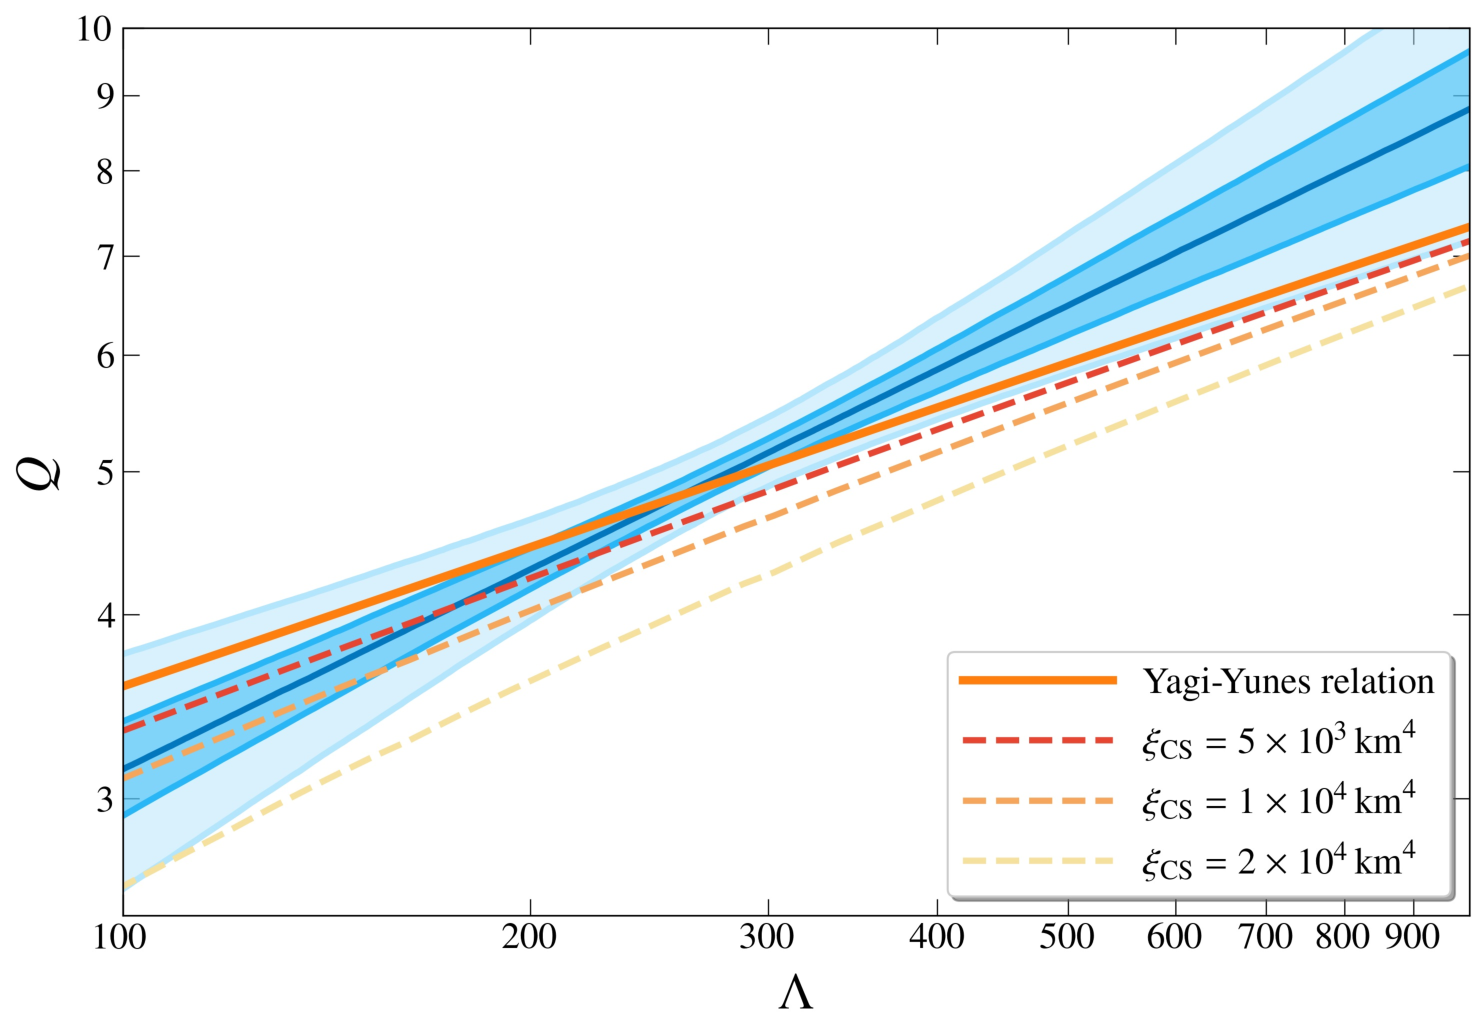
\includegraphics[width=\linewidth]{CS_xi_cs_AP4_2d.pdf}
    \end{minipage}
    \vspace{3mm}
    \begin{minipage}{0.48\linewidth}
        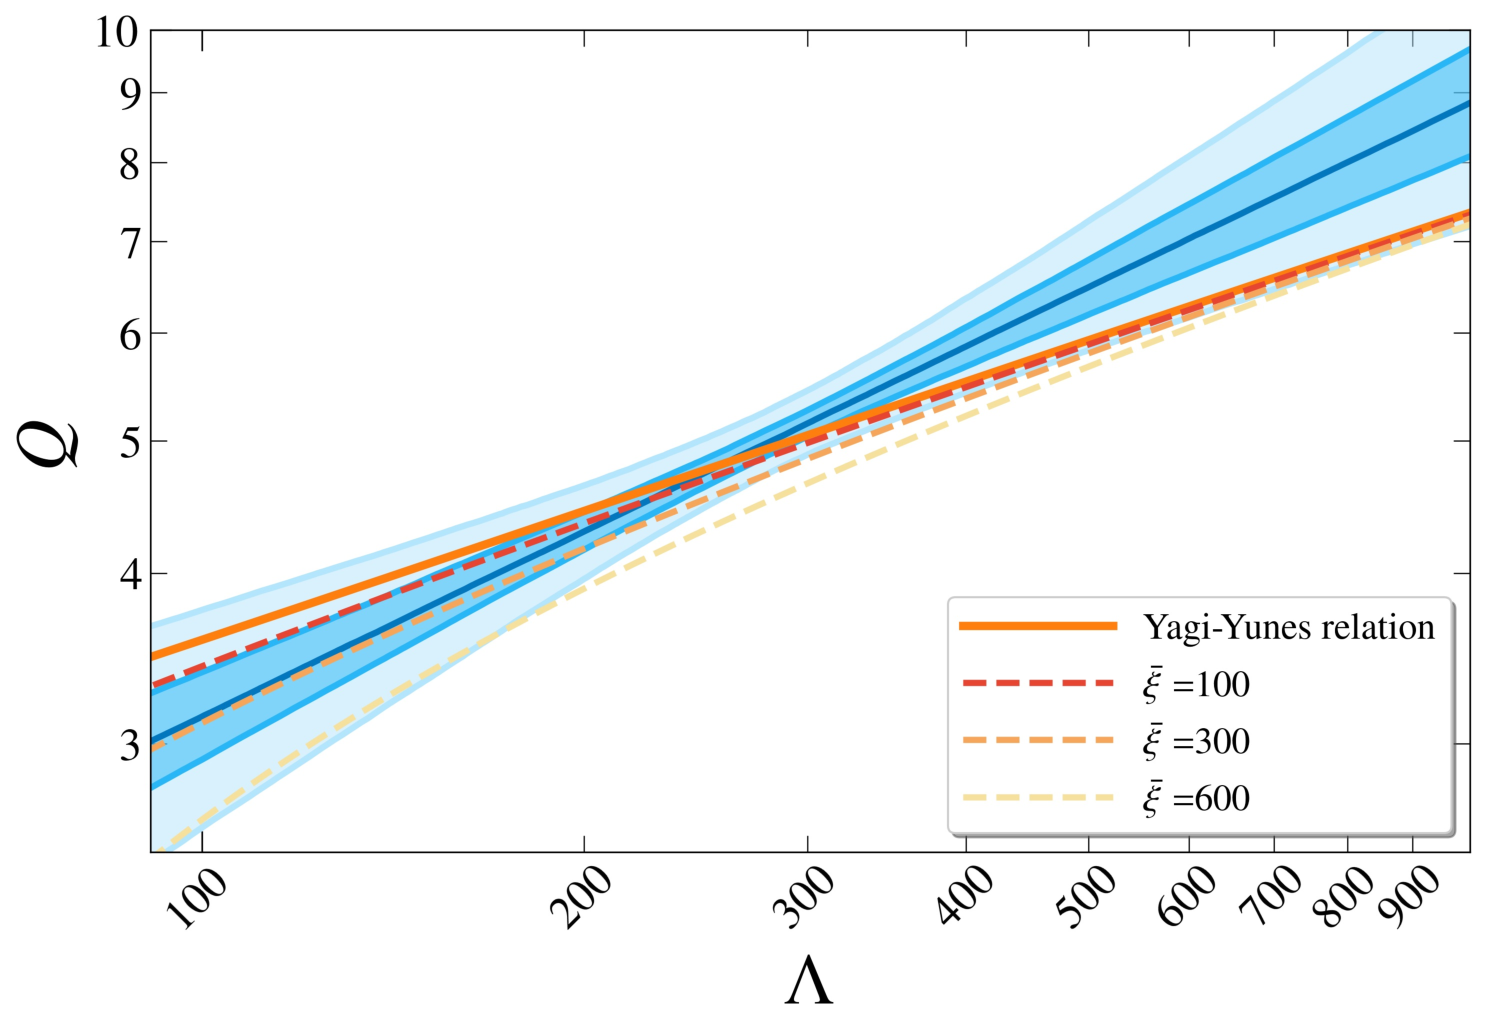
\includegraphics[width=\linewidth]{CS_xi_bar_AP4_2d.pdf}
    \end{minipage}
    \caption{Comparison of the hierarchical inference results and CS predictions with different coupling constants fixed. The blue regions are the same as figure~\ref{2-d_Love_Q} (Linear fitting model). For each of the coupling constants of CS gravity $\zeta, \xi_{\mathrm{CS}}$ and $\bar\xi$, three possible values are taken and the corresponding Love-Q relations for AP4 EOS are drawn respectively as references.}
    \label{cs_Love_Q}
\end{figure}

For some parity-violating modified gravity theories that have not been stringently constrained yet, an I-Love-Q test can be powerful due to the significant difference in I-Love-Q relation emerging in these theories compared with GR prediction~\cite{Yagi_2017, Yunes:2025xwp}. We select the dynamical Chern-Simons (dCS) gravity~\cite{Jackiw:2003pm, Smith:2007jm, Alexander:2009tp}, which is well-motivated from heterotic superstring theory~\cite{Polchinski:1998rq, Polchinski:1998rr}, loop quantum gravity~\cite{Alexander:2004xd, Taveras:2008yf, Calcagni:2009xz} and effective field theories of inflation~\cite{Weinberg:2008hq}, for discussion. The dCS gravity predicts a Love-Q relation different from the one in GR for any finite value of the coupling constant~\cite{Yagi:2013bca, Yagi:2013awa, Gupta:2017vsl}. By comparing this difference with the uncertainty given by our inference results, we can see to what extent can our results constrain the coupling constants in dCS gravity at most. 

%The dCS gravity introduces parity violation and quadratic curvature terms into the action~\cite{Alexander:2009tp, Gupta:2017vsl}
%\begin{equation}
%    \label{cs_action}
%    S = \int \mathrm{d}^4 x \sqrt{-g}\left[ \kappa_g \mathcal{R} + \frac{\alpha}{4} \mathcal{\vartheta} \mathcal{R}_{\nu\mu\rho\sigma} {}^{*}\mathcal{R}^{\mu\nu\rho\sigma} - \frac{\beta}{2}(\nabla_{\mu}\mathcal{\vartheta}\nabla^{\mu}\mathcal{\vartheta}+2V(\mathcal{\vartheta})) + \mathcal{L}_{\mathrm{mat}}\right]\,,
%\end{equation}
%where $\mathcal{R}$ is the Ricci scalar, $\mathcal{L}_{\mathrm{mat}}$ is the matter Lagrangian density, $g$ is the determinant of the metric, $\kappa_g\equiv 1/(16\pi)$, and $\alpha$ and $\beta$ 
%are the coupling constants in dCS gravity. We assume that the pseudo-scalar field $\mathcal{\vartheta}$ is dimensionless, thus the quantity $\xi_{\mathrm{CS}}^{1/4} \equiv [\alpha^2/(\kappa\beta)]^{1/4}$ \

The dCS gravity has a characteristic length $\xi_{\mathrm{CS}}^{1/4}$, which has been constrained by current Solar System observations to $\xi_{\mathrm{CS}}^{1/4}< \mathcal{O}(10^8)$km~\cite{Ali-Haimoud:2011zme, Yagi:2012ya}. For a Love-Q test, ref.~\cite{Yagi:2013mbt} obtained the dCS correction to the NS quadrupole moment and ref.~\cite{Yagi:2011xp} indicates that the tidal deformability is the same as in GR at leading order in small coupling approximation $\zeta \equiv \xi_{\mathrm{CS}} M^2/R^6 \ll 1$, regarding the dCS gravity as an effective theory. Refs.~\cite{Yagi_2017, Yagi:2013mbt} have discussed the I-Love-Q relations under dCS gravity and find that the relations remain universal when we normalize the variables with respect to $\bar{\xi}\equiv \xi_{\mathrm{CS}}/M^4$, while become EOS-sensative with $\xi_{\mathrm{CS}}$ or $\zeta$ fixed. 

Following ref.~\cite{Yagi_2017}, we calculate the dCS Love-Q relation with $\zeta, \xi_{\mathrm{CS}}$ and $\bar{\xi}$ fixed respectively assuming the AP4 EOS, which has been assumed in our simulation in section~\ref{sec3}. The results are demonstrated in figure~\ref{cs_Love_Q}. We compare the hierarchical Bayesian inference constraint of the Love-Q relation using linear fitting model (figure~\ref{2-d_Love_Q}) with some possible Love-Q relations with respect to certain coupling constants in dCS gravity. From figure~\ref{cs_Love_Q} we can conclude that our Love-Q test of dCS gravity can constrain the characteristic length $\xi_{\mathrm{CS}}^{1/4} < \mathcal{O}(10^2)$km, which is in agreement  
with the results given by refs.~\cite{Yagi:2013bca, Yagi:2013awa}.

%=============================
\section{Conclusion}
\label{sec6}
%=============================

In this work we adopted a hierarchical Bayesian framework to estimate the Love-Q relation of NSs. By separating the single-event inferences and hyper-parameter inference, this framework manifests high computational efficiency and provides a sophisticated statistical method for hyper-parameter estimation. We applied this framework to simulated GW events for a next-generation detector network to examine the potential of constraining the Love-Q relation with GW observations. The results demonstrated that with the next-generation GW detector network, one can obtain a reliable measurement of the Love-Q relation through hierarchical Bayesian inference. We have also verified that the inference results of the hyper-parameters are dominated by events with the highest SNRs, which is consistent with the findings of ref.~\cite{Lackey:2014fwa}.

We then investigated the impact of different parameterizations for Love-Q relation on the inference. We found that constraint of the Love-Q relation is insensitive to the parameterization in the region where most data points gather.
Also, as shown by the posterior distributions, degeneracies between hyper-parameters exist in all cases studied. Furthermore, for all but the linear model, at least one hyper-parameter was poorly constrained, exhibiting wide and flat posterior. These results indicate that a two-parameter (linear) model is sufficient for our data volume (20 GW events).

Finally, as a practical application, we compared our inference results with the theoretical predictions of the dCS gravity. The Love-Q relation measurement precision of our hierarchical Bayesian inference allows us to place a constraint on the dCS characteristic length $\xi_{\mathrm{CS}}^{1/4} < \mathcal{O}(10^2)$km. This result is consistent with previous works~\cite{Yagi:2013bca, Yagi:2013awa} and highlights the power of the Love-Q relation inference for testing gravity theories.

Future: Bias, Waveform, Overlapping, Precession, Earth rotation, Isolated and Binary, Large data size, octupole moment 

%=============================
\acknowledgments

\clearpage

\bibliographystyle{JHEP}
% \bibliographystyle{unsrt}
\bibliography{HBAGW_jcap}
\end{document}
